%=========================================================
% Informe actualizado a partir del esquematico KiCad,
% el firmware y los ensayos de banco del 14/09/2026.
%=========================================================
\documentclass[conference]{IEEEtran}
\IEEEoverridecommandlockouts

\usepackage[T1]{fontenc}
\usepackage[utf8]{inputenc}
\usepackage[spanish,es-noquoting]{babel}
\usepackage{graphicx}
\usepackage{amsmath,amssymb}
\usepackage{textcomp}
\usepackage{xcolor}
\usepackage{listings}
\usepackage{booktabs}
\usepackage{array}
\usepackage{tikz}
\usepackage{pdflscape}
\usetikzlibrary{arrows.meta,positioning,fit}

\definecolor{codegray}{gray}{0.95}
\definecolor{codegreen}{rgb}{0.0,0.45,0.0}
\definecolor{codeblue}{rgb}{0.0,0.0,0.6}
\lstset{
  language=C,
  basicstyle=\ttfamily\scriptsize,
  keywordstyle=\color{codeblue}\bfseries,
  commentstyle=\color{codegreen}\itshape,
  backgroundcolor=\color{codegray},
  numbers=none,
  breaklines=true,
  frame=single,
  framerule=0pt,
  captionpos=b,
  columns=fullflexible,
  aboveskip=4pt,
  belowskip=4pt
}

\begin{document}

\title{Fuente conmutada elevadora de dos ramas independientes\\
\large Control con FreeRTOS e integración con GNU/Linux}

\author{
\IEEEauthorblockN{Brian Benavidez}
\IEEEauthorblockA{Ingeniería Electrónica -- Universidad Tecnológica Nacional\\
Buenos Aires, Argentina\\
Brianandres99@gmail.com}
}

\maketitle

\begin{abstract}
Se presenta una fuente partida con salidas positiva y negativa regulables de forma independiente entre 0 y 30~V, con límite de corriente configurable hasta 0,75~A por rama. Una Raspberry Pi Pico 2W genera dos PWM de 50~kHz y ejecuta el control, la adquisición y las protecciones mediante FreeRTOS. La ampliación EGB incorpora comunicación con GNU/Linux por UART, un controlador de carácter basado en \textit{serdev} y dos aplicaciones de usuario: una herramienta de consola y un panel web. La arquitectura conserva el control de tiempo real en el microcontrolador y delega supervisión y configuración al sistema Linux. Se documentan el diseño electrónico, la calibración, las protecciones y la verificación integral del enlace.
\end{abstract}

\begin{IEEEkeywords}
Fuente partida, convertidor flyback, PWM, control PI, FreeRTOS, RP2350, ADS1115, Linux, controlador de dispositivo, UART.
\end{IEEEkeywords}

\newpage
{\small\setcounter{tocdepth}{1}\tableofcontents}
\clearpage

%=========================================================
\section{Introducción}

El objetivo del proyecto es obtener dos tensiones continuas respecto de una masa común: una positiva y otra negativa. Ambas salidas se configuran, miden, habilitan y protegen de manera independiente. La etapa de entrada admite tensiones entre 3,7 y 15~V.

La placa utiliza dos ramas tipo \textit{flyback} no aisladas, ya que los secundarios comparten GND con el control. Cada rama posee regulación, medición, habilitación y protección independientes. La entrada de diseño es de 3,7 a 15~V, la referencia alcanza 30~V y se adopta 750~mA como máximo conservador por rama.

Para un convertidor \textit{flyback} ideal, la magnitud de salida puede aproximarse por

\begin{equation}
\left|\frac{V_o}{V_i}\right| \approx \frac{N_s}{N_p}\frac{D}{1-D},
\label{eq:flyback}
\end{equation}

donde $N_s/N_p$ es la relación de espiras y $D$ el ciclo de trabajo. En el prototipo la relación es aproximadamente 2:1. La ecuación sólo sirve como referencia inicial: las caídas en semiconductores, la resistencia de los bobinados, la carga, el acoplamiento y las pérdidas del núcleo modifican considerablemente el resultado real. Por ese motivo se implementó regulación por realimentación.

%=========================================================
\section{Descripción de los módulos de hardware principales}

La Fig.~\ref{fig:bloques_detallado}, incluida en los apéndices, resume los bloques del circuito implementado y los pines utilizados entre la Pico y los módulos. Las ramas se controlan llevando su PWM a cero o aplicando el ciclo calculado.

\subsection{Raspberry Pi Pico 2W}

La Raspberry Pi Pico 2W, basada en el RP2350, genera ambos PWM, mide Vin y las corrientes, recibe por I$^2$C las tensiones del ADS1115 y gestiona encoders, LCD, UART y flash. FreeRTOS separa adquisición, control e interfaz; el corte rápido por sobrecorriente se realiza desde la interrupción del ADC.

\begin{figure}[!ht]
\centering
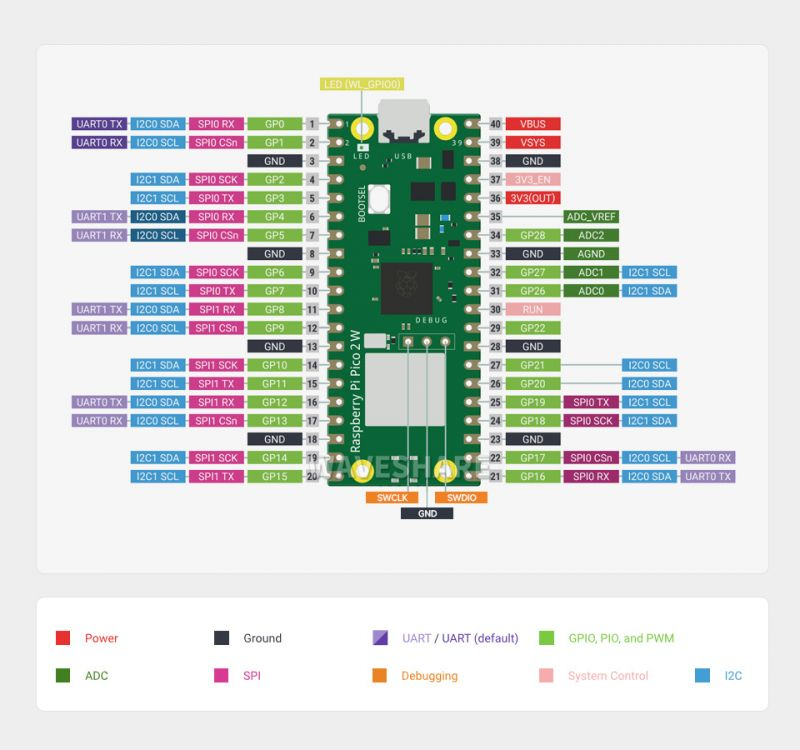
\includegraphics[width=0.94\columnwidth,height=0.20\textheight,keepaspectratio]{pico2w_pinout.jpg}
\caption{Raspberry Pi Pico 2W y distribución de pines empleada como referencia para la asignación de señales.}
\label{fig:pico_pinout}
\end{figure}

\subsection{Módulo S09 y conexión USB}

El módulo U4 S09, con convertidor marcado B6285, genera +5~V para VSYS y el TC4427. Los 3,3~V de la Pico alimentan el MCP6004 y el ADS1115. VBUS está separado del riel +5~V y de VCC, por lo que el USB puede coexistir con la alimentación externa si se conserva una masa común.

\begin{figure}[!ht]
\centering
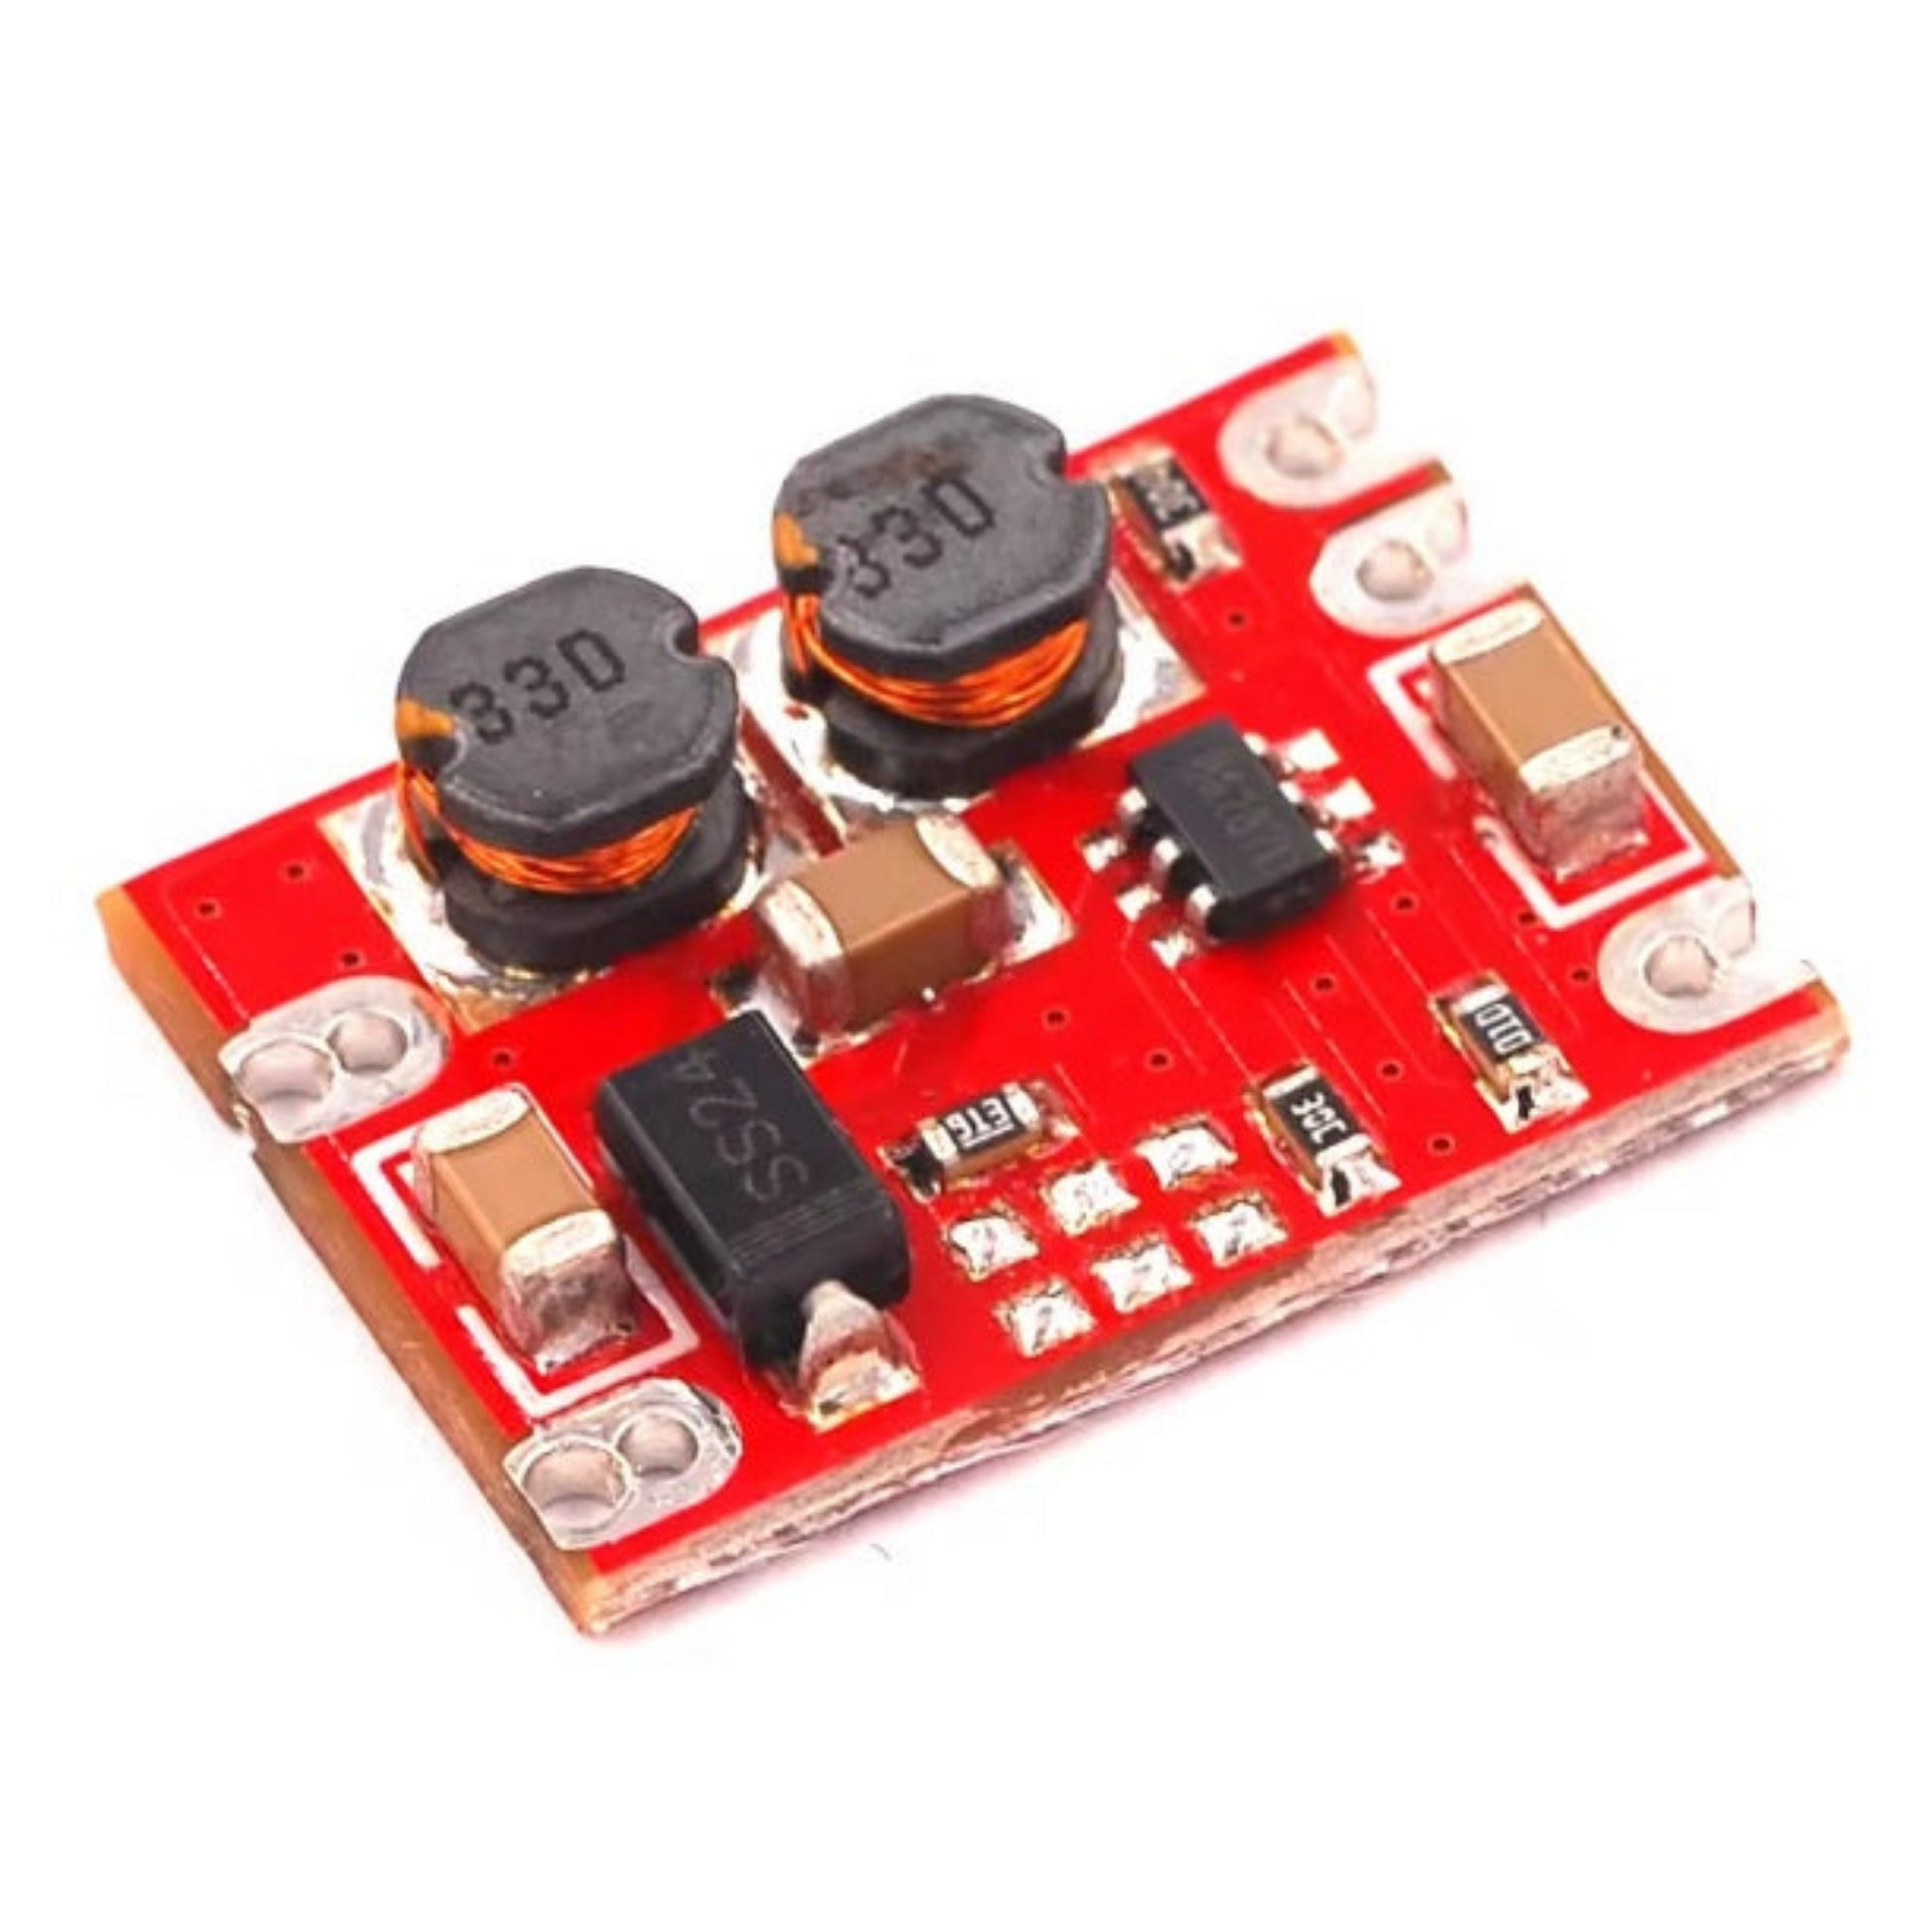
\includegraphics[width=0.82\columnwidth,height=0.19\textheight,keepaspectratio]{s09_module_real.jpg}
\caption{Fotografía del módulo S09, con sus dos inductores y la etapa convertidora utilizada para generar el riel auxiliar de 5~V \cite{web_s09}.}
\label{fig:s09}
\end{figure}

\subsection{Conversor ADS1115}

El módulo ADS1115 realiza la adquisición de las tensiones positiva y negativa con resolución de 16~bits. Se conecta al mismo bus I$^2$C0 del LCD, utiliza la dirección 0x48 y entrega al firmware las muestras de AIN0 y AIN1 para su posterior conversión y calibración.

\begin{figure}[!ht]
\centering
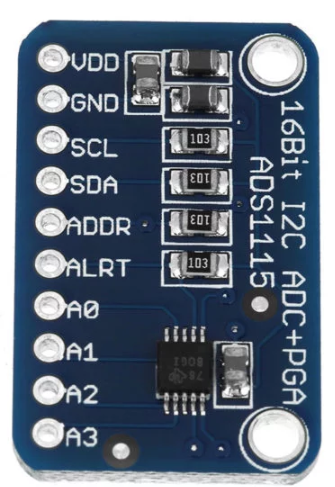
\includegraphics[width=0.48\columnwidth,height=0.17\textheight,keepaspectratio]{ads1115_module_blue.png}
\caption{Módulo ADS1115 instalado en el prototipo.}
\label{fig:ads1115_modulo}
\end{figure}

\subsection{Interfaz LCD con PCF8574}

El LCD 20$\times$4 se conecta mediante un módulo PCF8574 configurado en la dirección 0x27. Comparte el bus I$^2$C0 con el ADS1115 a través de GPIO12 (SDA) y GPIO13 (SCL); el acceso al bus se coordina en firmware mediante un mutex.

\begin{figure}[!ht]
\centering
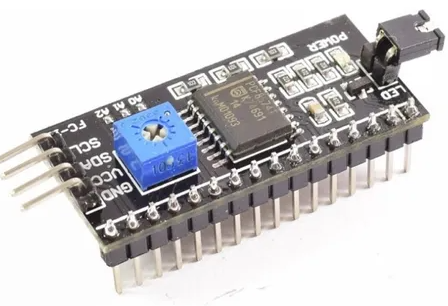
\includegraphics[width=0.92\columnwidth,height=0.19\textheight,keepaspectratio]{pcf8574_module.png}
\caption{Interfaz PCF8574 empleada por el LCD 20$\times$4.}
\label{fig:pcf8574}
\end{figure}

\subsection{Etapas de potencia}

Las dos ramas utilizan los mismos elementos principales y difieren en la polaridad del secundario y del rectificador. La Tabla~\ref{tab:potencia} reúne los valores extraídos del esquemático de KiCad.

\begin{table}[!t]
\caption{Elementos principales de la placa implementada}
\label{tab:potencia}
\centering
\footnotesize
\begin{tabular}{@{}lll@{}}
\toprule
\textbf{Elemento} & \textbf{Rama positiva} & \textbf{Rama negativa} \\
\midrule
MOSFET & Q1 FQP30N06L & Q2 FQP30N06L \\
Transformador & TR1 100/400~$\mu$H & TR2 100/400~$\mu$H \\
Rectificador & D1 UF4007 & D4 UF4007 \\
Diodo de \textit{snubber} & D3 STPS10H100C & D5 STPS10H100C \\
Red RC & R3 3,9~k$\Omega$, C3 100~nF & R14 3,9~k$\Omega$, C8 100~nF \\
Capacitor de salida & C4 1000~$\mu$F/50~V & C9 1000~$\mu$F/50~V \\
Shunt & 0,1~$\Omega$/2~W & 0,1~$\Omega$/2~W \\
Conector & J2 VOUT\_POS & J6 VOUT\_NEG \\
\bottomrule
\end{tabular}
\end{table}

\subsection{Driver dual TC4427}

U3 es un driver doble no inversor. Recibe PWM\_POS y PWM\_NEG desde GPIO16 y GPIO17 y excita las compuertas con casi 5~V. En banco se midieron 4,96~V de alimentación y se observaron ambos PWM en sus salidas.

\subsection{MOSFET FQP30N06L}

Q1 y Q2 son FQP30N06L de 60~V. Cada compuerta posee 15~$\Omega$ en serie y 10~k$\Omega$ a fuente. Después del ajuste del \textit{snubber} se observó un pico de VDS cercano a 40~V.

\subsection{Transformadores TR1 y TR2}

TR1 y TR2 poseen 32 vueltas primarias y 64 secundarias con alambre de 0,6~mm, núcleo E--E y \textit{gap} total aproximado de 1~mm. Se midieron 99,9~$\mu$H y 413,7~$\mu$H. La polaridad secundaria se invierte entre ramas para obtener los dos signos; no existe aislamiento galvánico porque comparten GND.

Cada primario incorpora una red RCD de limitación de transitorios. Durante las pruebas, un capacitor cerámico marcado 223 se dañó. Se ensayaron otros valores y la versión reflejada en el esquemático utiliza 100~nF/100~V. Con esta modificación se observó un pico de VDS cercano a 40~V alrededor de 15~\% de \textit{duty}; antes se habían observado picos de aproximadamente 47~V.

%=========================================================
\section{Adquisición y acondicionamiento analógico}

\subsection{Configuración y conversión del ADS1115}

U2 posee cuatro entradas analógicas y amplificador de ganancia programable. ADDR se conecta a GND, por lo que la dirección utilizada es 0x48. El firmware selecciona el rango de $\pm4,096$~V y una velocidad de 860 muestras/s.

AIN0 mide VSENSE\_POS y AIN1 VSENSE\_NEG; AIN2 y AIN3 quedan libres. Cada lectura se realiza en modo \textit{single-shot} y devuelve un entero con signo de 16~bits.

La conversión del código a la tensión presente en el pin se realiza mediante

\begin{equation}
V_{AIN}=\frac{\text{raw}\cdot(2\cdot4,096)}{2^{16}}
=\frac{\text{raw}\cdot4,096}{2^{15}}.
\end{equation}

\subsection{Amplificador operacional MCP6004}

U1 es un MCP6004 cuádruple alimentado con 3,3~V. Sus cuatro amplificadores se encuentran ocupados: U1B acondiciona Vout positiva, U1C invierte y atenúa Vout negativa, U1A amplifica la caída del shunt positivo y U1D invierte y amplifica la del shunt negativo. No queda una sección disponible como comparador de protección.

El MCP6004 permite presentar señales positivas a los ADC aun cuando la salida de potencia sea negativa. Todas sus entradas y salidas deben mantenerse dentro de los rieles de 0 y 3,3~V.

\subsection{Asignación de mediciones}

La asignación empleada por la PCB y por el firmware es la siguiente:

\begin{table}[!t]
\caption{Canales analógicos utilizados}
\label{tab:analogicos}
\centering
\footnotesize
\begin{tabular}{@{}lll@{}}
\toprule
\textbf{Magnitud} & \textbf{Entrada} & \textbf{Origen} \\
\midrule
$V_{in}$ & GPIO26 / ADC0 & divisor R1--R4 \\
$I_{out-}$ & GPIO27 / ADC1 & ISENSE\_NEG \\
$I_{out+}$ & GPIO28 / ADC2 & ISENSE\_POS \\
$V_{out+}$ & ADS1115 AIN0 & VSENSE\_POS \\
$|V_{out-}|$ & ADS1115 AIN1 & VSENSE\_NEG \\
\bottomrule
\end{tabular}
\end{table}

El ADS1115 sólo mide las dos tensiones de salida. Las corrientes se leen con el ADC interno para reducir la latencia de la protección de sobrecorriente.

\subsection{Tensión de entrada}

R1=10~k$\Omega$ y R4=2,2~k$\Omega$ forman un divisor conectado a ADC0. El firmware reconstruye la tensión mediante

\begin{equation}
V_{in,calc}=V_{ADC}\frac{10\,000+2\,200}{2\,200}.
\end{equation}

El diodo Zener D2 (1N4728) limita la tensión del nodo VIN\_SENSE. Para 15~V de entrada el ADC recibe aproximadamente 2,70~V.

\subsection{Tensiones de salida}

La salida positiva se atenúa con R2=330~k$\Omega$ y R6=22~k$\Omega$. U1B funciona como seguidor y R5--C6 (4,7~k$\Omega$/100~nF) filtra la señal antes de AIN0. La reconstrucción previa a la calibración es

\begin{equation}
V_{out+,calc}=V_{AIN0}\frac{330+22}{22}=16V_{AIN0}.
\end{equation}

La salida negativa se convierte en una magnitud positiva mediante U1C, R13=820~k$\Omega$ y R12=51~k$\Omega$. R15--C11 aplica el mismo filtro de 4,7~k$\Omega$/100~nF antes de AIN1:

\begin{equation}
|V_{out-,calc}|=V_{AIN1}\frac{820}{51}.
\end{equation}

\subsection{Corrientes}

Cada salida posee un shunt de 0,1~$\Omega$/2~W. U1A amplifica la corriente positiva con ganancia no inversora $1+200/22=10,09$. U1D acondiciona la corriente negativa con una ganancia de magnitud $220/22=10$. Por lo tanto, las sensibilidades nominales son aproximadamente 1,009~V/A y 1,000~V/A. R9--C7 y R20--C12 filtran las señales antes de ADC2 y ADC1.

La corriente máxima adoptada es de 750~mA por rama debido al UF4007 y al margen requerido frente a corriente de pico y temperatura. El ajuste comienza en 0,1~A y no debe superar 0,75~A.

%=========================================================
\section{Calibración de las mediciones}

La calibración se aplica después de convertir el código del ADC a tensión y después de deshacer el divisor o la ganancia analógica. Es decir, la tabla no recibe directamente el valor crudo del ADS1115.

El recorrido completo es

\begin{equation}
\text{ADC crudo}\rightarrow V_{pin}\rightarrow V_{calc}\rightarrow V_{calibrada}.
\end{equation}

En cada tabla, la primera columna contiene el valor calculado que el sistema habría mostrado sin corrección y la segunda representa la tensión real medida con el osciloscopio respecto de GND. El algoritmo localiza los dos puntos vecinos e interpola linealmente:

\begin{equation}
V=V_{r1}+\frac{V_{calc}-V_{c1}}{V_{c2}-V_{c1}}(V_{r2}-V_{r1}).
\label{eq:interpolacion}
\end{equation}

\begin{lstlisting}[caption={Interpolación lineal utilizada por las tablas de salida.}]
while (upper < count && measured_volts > points[upper].measured_volts) upper++;
if (upper == count) upper = count - 1U;
float fraction = (measured_volts - points[upper - 1U].measured_volts) / (points[upper].measured_volts - points[upper - 1U].measured_volts);
float calibrated = points[upper - 1U].real_volts + fraction * (points[upper].real_volts - points[upper - 1U].real_volts);
\end{lstlisting}

Las tablas se encuentran en \texttt{vin\_calibration.h}, \texttt{vout\_pos\_calibration.h} y \texttt{vout\_neg\_calibration.h}. Los puntos de salida están espaciados 0,5~V; entre ellos se interpola y, por encima del último, se extrapola con el tramo final.

Las salidas se midieron respecto de GND, después de los shunts. Por ello cada tabla corrige la cadena completa de su rama y no puede intercambiarse con la otra. Para obtener y verificar los puntos se utilizaron un osciloscopio Hantek DSO2D10 y un multímetro \textit{True RMS} Gralf GMF-39D; la fuente de laboratorio aportó las lecturas de tensión y corriente de entrada. El multímetro también se empleó para comprobar las resistencias de carga y las caídas sobre los shunts. La verificación final presentó un apartamiento máximo cercano a 0,1~V alrededor de 12,5~V. La Fig.~\ref{fig:antes_calibracion} muestra el banco antes de aplicar esta corrección.

%=========================================================
\section{Dimensionamiento de la etapa de potencia}

\subsection{Relación de transformación}

Con 32 vueltas primarias y 64 secundarias se obtiene $N_s/N_p=2$. La relación $413,7/99,9\approx4,14$ entre inductancias concuerda con $(64/32)^2=4$. El PI ajusta el ciclo porque la salida real también depende de pérdidas, carga, Vin y acoplamiento.

\subsection{Redes snubber}

R3--C3--D3 y R14--C8--D5 forman las redes RCD asociadas a los primarios. El capacitor absorbe parte de la energía del pico, el diodo dirige el transitorio hacia la red y la resistencia disipa la energía almacenada. Aumentar el capacitor reduce el pico pero incrementa la energía que debe manejar la resistencia y puede aumentar las pérdidas. El valor actual de 100~nF fue elegido de forma experimental.

%=========================================================
\section{Firmware}

\subsection{Periféricos y pines}

\begin{table}[!t]
\caption{Asignación digital de la Pico 2W}
\label{tab:pines}
\centering
\footnotesize
\begin{tabular}{@{}ll@{}}
\toprule
\textbf{Función} & \textbf{GPIO} \\
\midrule
UART0 TX / RX & 0 / 1 \\
Encoder positivo CLK / DT / SW & 2 / 3 / 4 \\
Encoder negativo CLK / DT / SW & 6 / 7 / 8 \\
I$^2$C0 SDA / SCL & 12 / 13 \\
PWM positivo / negativo & 16 / 17 \\
ADC Vin / I- / I+ & 26 / 27 / 28 \\
\bottomrule
\end{tabular}
\end{table}

El LCD y el ADS1115 comparten I$^2$C0 a 100~kHz. El ADS1115 utiliza dirección 0x48, PGA de $\pm4,096$~V y 860 muestras/s en modo \textit{single-shot}. La UART trabaja a 115200~bit/s.

\subsection{Organización en tareas}

El programa crea siete tareas. Una misma función de control se instancia dos veces, una por rama, y cada instancia conserva su referencia, integrador, habilitación, límites y fallas. La tarea \texttt{protection\_task} se mantiene separada de la adquisición calibrada porque selecciona en forma secuencial los tres canales del ADC interno y atiende la supervisión rápida de corriente y de Vin.

\begin{table}[!t]
\caption{Tareas de FreeRTOS}
\label{tab:tareas}
\centering
\scriptsize
\begin{tabular}{@{}llll@{}}
\toprule
\textbf{Tarea} & \textbf{Prio.} & \textbf{Período} & \textbf{Función} \\
\midrule
\texttt{protection\_task} & 5 & 1 ms & ADC interno y protección \\
\texttt{adc\_task} & 3 & 5 ms & ADS1115 y publicación \\
\texttt{control\_task} & 4 & 5 ms & PI positivo \\
\texttt{control\_task} & 4 & 5 ms & PI negativo \\
\texttt{encoder\_task} & 3 & 1 ms & Interfaz local \\
\texttt{uart\_task} & 2 & 2 ms & Protocolo UART \\
\texttt{display\_task} & 1 & 100 ms & Actualización del LCD \\
\bottomrule
\end{tabular}
\end{table}

El bus I$^2$C se protege con un mutex. Las mediciones, consignas, estados y fallas se copian dentro de secciones críticas breves para formar una instantánea coherente. La interrupción del FIFO del ADC corta directamente el PWM si detecta sobrecorriente y no espera la ejecución de una tarea.

Las tareas se crean de forma explícita en \texttt{main}; así puede observarse qué función ejecuta cada una y con qué prioridad:

\begin{lstlisting}[caption={Creación de las siete tareas del programa principal.}]
xTaskCreate(protection_task, "PROTECTION", TASK_STACK_PROTECTION_WORDS, NULL, TASK_PRIORITY_PROTECTION, NULL);
xTaskCreate(adc_task, "ADC", TASK_STACK_ADC_WORDS, NULL, TASK_PRIORITY_ADC, NULL);
xTaskCreate(control_task, "CONTROL", TASK_STACK_CONTROL_WORDS, NULL, TASK_PRIORITY_CONTROL, NULL);
xTaskCreate(control_task, "CONTROL2", TASK_STACK_CONTROL2_WORDS, (void *)1, TASK_PRIORITY_CONTROL2, NULL);
xTaskCreate(encoder_task, "ENCODER", TASK_STACK_ENCODER_WORDS, NULL, TASK_PRIORITY_ENCODER, NULL);
xTaskCreate(uart_task, "UART", TASK_STACK_UART_WORDS, NULL, TASK_PRIORITY_UART, NULL);
xTaskCreate(display_task, "DISPLAY", TASK_STACK_DISPLAY_WORDS, NULL, TASK_PRIORITY_DISPLAY, NULL);
vTaskStartScheduler();
\end{lstlisting}

La Fig.~\ref{fig:tareas} muestra por separado las funciones de cada tarea, su prioridad y los recursos compartidos que utiliza.

\subsection{Tarea de medición}

\texttt{protection\_task} se ejecuta cada 1~ms. Selecciona sucesivamente Vin, I$-$ e I$+$, descarta dos conversiones después de cada cambio de canal y promedia cuatro muestras válidas. Este procedimiento evita que el asentamiento del multiplexor mezcle el valor de un canal con el siguiente. \texttt{adc\_task}, cada 5~ms, toma esas lecturas internas, adquiere V$+$ y V$-$ desde el ADS1115, convierte las cinco magnitudes y publica el conjunto calibrado para las demás tareas.

\subsection{Control PI y PWM}

GPIO16 y GPIO17 pertenecen al mismo \textit{slice} PWM, por lo que ambas ramas comparten una frecuencia de 50~kHz y utilizan canales diferentes. El ciclo se limita entre 0 y 70~\%.

Cada lazo ejecuta

\begin{equation}
D=K_p e+K_i\int e\,dt, \qquad e=V_{ref}-V_o,
\end{equation}

con $K_p=0,80$, $K_i=2,00$ y término derivativo nulo. El término integral se limita al intervalo equivalente al rango útil del PWM, evitando que crezca sin control cuando la salida alcanza su máximo.

La frecuencia y los límites principales se encuentran juntos al comienzo del archivo:

\begin{lstlisting}[caption={Parámetros principales de PWM y control.}]
#define PWM_FREQUENCY_HZ 50000U
#define DUTY_MIN_PERCENT 0.0f
#define DUTY_MAX_PERCENT 70.0f
#define SOFT_START_TIME_SECONDS 2.00f
#define PID_KP 0.80f
#define PID_KI 2.00f
\end{lstlisting}

Al habilitar una rama, su referencia interna sube desde cero hasta el valor pedido durante 2~s. Si la medición deja de ser válida, la salida se deshabilita o existe una falla enclavada, el PWM correspondiente pasa a cero y su integrador se reinicia.

\subsection{Protecciones digitales}

Durante las conversiones válidas de I$-$ e I$+$, cada muestra ingresa al FIFO y genera una interrupción. Si una corriente supera su límite ajustado, el manejador enclava la falla y lleva inmediatamente a cero el PWM de la rama afectada. Luego, \texttt{protection\_task} actualiza el estado de habilitación que utilizan la pantalla y el resto del programa. La misma tarea compara muestras consecutivas de Vin y apaga ambas ramas si detecta una caída brusca compatible con una sobrecorriente en la entrada.

La sobretensión se comprueba al adquirir cada tensión con el ADS1115. Si la lectura calibrada supera el límite de su rama, se enclava la falla y su PWM se lleva a cero. El límite de sobretensión puede configurarse entre 5 y 40~V; la referencia se limita entre 5 y 30~V.

Estas protecciones son digitales. La sobrecorriente no espera a una tarea de FreeRTOS; su tiempo de respuesta queda determinado por el muestreo del ADC y la ejecución de la interrupción. La PCB no posee un comparador analógico dedicado ni un apagado puramente asíncrono.

\begin{lstlisting}[caption={Corte inmediato desde la interrupción del ADC.}]
if (adc_active_channel == IOUT1_ADC_CHANNEL && actual_duty_percent > 0.0f && raw >= overcurrent_raw_limit) {
    overcurrent_fault_latched = true;
    pwm_set_chan_level(pwm_gen_slice, pwm_gen_channel, 0U);
    actual_duty_percent = 0.0f;
}
\end{lstlisting}

Al detectarse una falla se pone en cero el canal PWM correspondiente y se deshabilita la salida afectada. Después de retirar la causa, una pulsación larga del encoder limpia la falla sin volver a encender la rama.

\subsection{Encoders y LCD}

Cada encoder controla exclusivamente su rama. El giro modifica el parámetro seleccionado; una pulsación corta recorre referencia de tensión, límite de corriente, límite de sobretensión y visualización del PWM. Una pulsación larga habilita o apaga la salida, siempre que no exista una falla enclavada.

El LCD conserva dos columnas: la rama negativa se presenta a la izquierda y la positiva a la derecha, en concordancia con la disposición mecánica de los encoders y bornes. La primera fila muestra Vin y los estados ON/OFF; la segunda, V$-$ y V$+$; la tercera, I$-$ e I$+$; y la cuarta muestra el parámetro seleccionado de cada encoder. Ante una falla aparecen \texttt{OV} o \texttt{OC} en la posición de la rama afectada.

El LCD 20$\times$4 utiliza un PCF8574 en la dirección 0x27 y comparte I$^2$C0 con el ADS1115 mediante un mutex. Los KY-040 se sondean cada 1~ms; la biblioteca \texttt{encoder} resuelve la cuadratura, el antirrebote y las pulsaciones corta y larga.

\subsection{Memoria flash}

El módulo \texttt{settings\_storage} guarda seis valores: referencia, límite de corriente y límite de sobretensión de cada rama. El registro se almacena en el último sector de la flash e incluye firma, versión y suma de verificación. El guardado se solicita con el comando \texttt{SAVE} y sólo se acepta cuando las dos salidas están apagadas. Los estados ON/OFF no se guardan, por lo que el equipo siempre inicia con ambas ramas deshabilitadas.

\begin{lstlisting}[caption={Datos persistentes almacenados por cada rama.}]
typedef struct {
    float voltage_positive;
    float voltage_negative;
    float current_positive;
    float current_negative;
    float overvoltage_positive;
    float overvoltage_negative;
} stored_settings_t;
\end{lstlisting}

Antes de programar la flash, el firmware fuerza ambos PWM a cero, borra el último sector y escribe una página con la firma, la versión, los seis valores y la suma de verificación.

\subsection{Comunicación UART}

El conector J13 utiliza UART0, TX en GPIO0, RX en GPIO1 y GND. Los comandos implementados son:

\begin{itemize}
\item \texttt{GET}: devuelve tensiones, corrientes, referencias y estados.
\item \texttt{SET P 12.5} o \texttt{SET N 12.5}: cambia la referencia indicada.
\item \texttt{SET ILP 0.50} o \texttt{SET ILN 0.50}: cambia el límite de corriente.
\item \texttt{SET VLP 32.0} o \texttt{SET VLN 32.0}: cambia el límite de sobretensión.
\item \texttt{OUT P ON/OFF} o \texttt{OUT N ON/OFF}: controla una rama.
\item \texttt{RESET P} o \texttt{RESET N}: borra la falla enclavada y mantiene la salida apagada.
\item \texttt{SAVE}: guarda la configuración si ambas ramas están apagadas.
\end{itemize}

\begin{lstlisting}[caption={Ejemplos de comunicación con otra placa.}]
GET
SET P 12.5
SET ILN 0.50
SET VLP 32.0
OUT P ON
RESET N
SAVE
\end{lstlisting}

Cada comando se procesa al recibir una nueva línea. Si el terminal envía la secuencia \texttt{CRLF}, el retorno de carro se ignora y el comando se ejecuta al recibir \texttt{LF}. Las respuestas comienzan con \texttt{OK} o \texttt{ERR}; el comando \texttt{GET} devuelve en una sola línea el estado de las dos ramas.

%=========================================================
\section{Integración EGB con GNU/Linux}

La ampliación EGB conecta la UART de la placa con un sistema GNU/Linux. El microcontrolador continúa ejecutando el lazo PI, el muestreo y el corte rápido de las salidas; Linux sólo envía comandos y presenta la información al usuario. Esta separación evita que la latencia del sistema operativo afecte las funciones críticas de control y protección.

\subsection{Arquitectura de software}

La Fig.~\ref{fig:arquitectura_egb} muestra las capas implementadas. El \textit{Device Tree overlay} declara el dispositivo conectado al UART. El controlador del kernel se enlaza mediante \textit{serdev}, registra el dispositivo de carácter \texttt{/dev/ega\_uart} y entrega a espacio de usuario la misma interfaz de lectura y escritura para ambas aplicaciones.

\begin{figure*}[!t]
\centering
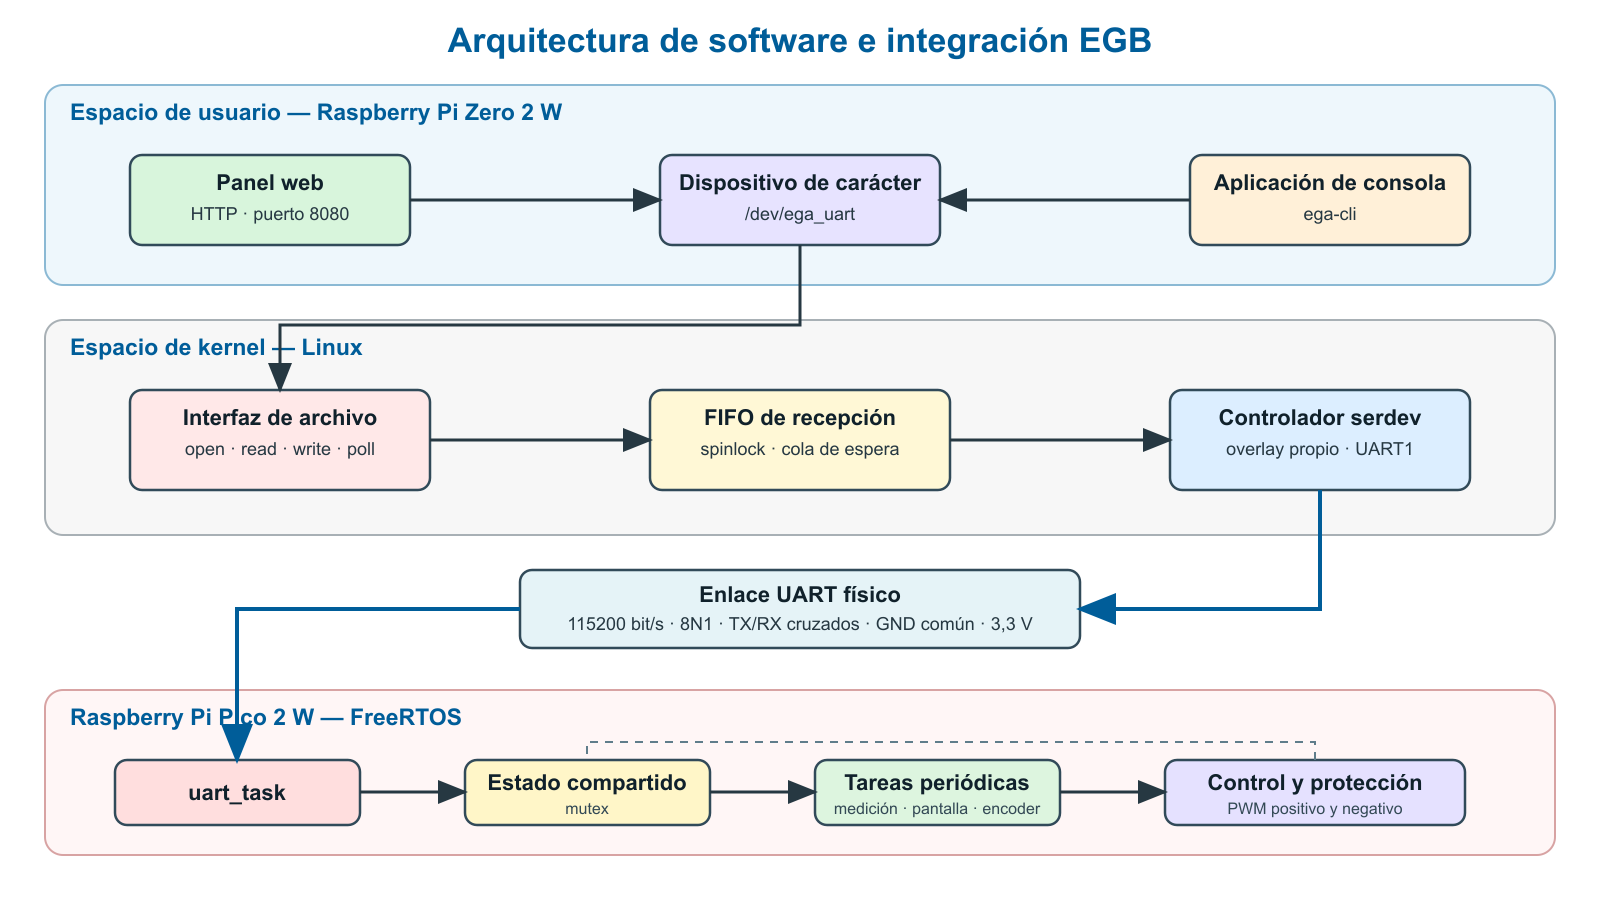
\includegraphics[width=0.88\textwidth,height=0.31\textheight,keepaspectratio]{arquitectura_egb.png}
\caption{Arquitectura de la EGB desde las aplicaciones de usuario hasta el firmware de la fuente.}
\label{fig:arquitectura_egb}
\end{figure*}

El camino de transmisión es aplicación--\texttt{write()}--controlador--UART--Pico. En recepción, la rutina de \textit{serdev} deposita los bytes en un \texttt{kfifo}; una cola de espera bloquea la lectura hasta disponer de datos. Un \textit{spinlock} protege el FIFO dentro del contexto de recepción y un mutex serializa cada transacción completa, de modo que dos procesos no mezclen comandos y respuestas. La desconexión despierta a los lectores y evita que queden bloqueados sobre un dispositivo inexistente.

\subsection{Aplicaciones de usuario}

La aplicación de consola, escrita en C, permite una orden directa o una sesión interactiva. Valida localmente el formato básico, escribe el comando en \texttt{/dev/ega\_uart}, espera la respuesta y la presenta sin interpretar decisiones de control.

El panel web se ejecuta como un servicio local en Python y utiliza únicamente la biblioteca estándar. Publica el estado de las dos ramas, las mediciones, las consignas y las fallas; además permite modificar referencias y límites, habilitar o apagar salidas, borrar fallas y solicitar el guardado. Su servidor acepta peticiones HTTP locales y reutiliza el mismo protocolo textual, por lo que no introduce un segundo camino de control.

\subsection{Alcance de la interfaz}

Los límites aplicados por la interfaz coinciden con el firmware: referencia de 0 a 30~V, corriente de 0,10 a 0,75~A y sobretensión de 5 a 40~V. El panel no reemplaza las comprobaciones del microcontrolador; si un valor no es válido o existe una falla, la Pico responde \texttt{ERR} y mantiene la salida en condición segura. El código, los archivos de compilación, el \textit{overlay}, la regla \textit{udev}, las aplicaciones y la documentación se encuentran disponibles en el repositorio académico del proyecto.

%=========================================================
\section{Diseño electrónico y PCB}

\subsection{Distribución funcional}

La etapa de control se concentra alrededor de la Pico, el MCP6004 y el ADS1115. Las pistas de sensado se mantienen alejadas de los nodos SW\_POS y SW\_NEG. Los transformadores, MOSFETs, rectificadores y capacitores de salida forman los lazos de potencia, mientras que el S09 queda próximo al sector de alimentación auxiliar.

La PCB implementada mide 150~mm por 100~mm. Es una placa principalmente monocapa en B.Cu; los cruces que no pueden resolverse en la cara inferior se implementan con puentes físicos. Las pistas de potencia son más anchas que las señales de control y el plano de masa reduce la impedancia de retorno.

\subsection{Lista de puntos de prueba}

Se incorporaron puntos de prueba para verificar el prototipo sin apoyar la sonda directamente sobre encapsulados próximos. La Tabla~\ref{tab:testpoints} identifica los conectores previstos en el esquemático.

\begin{table}[!t]
\caption{Conectores utilizados como puntos de prueba}
\label{tab:testpoints}
\centering
\footnotesize
\begin{tabular}{@{}lll@{}}
\toprule
\textbf{Conector} & \textbf{Señales} & \textbf{Uso} \\
\midrule
J7 & GND, +5~V, +3,3~V & Alimentación lógica \\
J8 & PWM$+$, PWM$-$ & Compuertas/driver \\
J9 & VSENSE$+$, VSENSE$-$ & Tensión acondicionada \\
J10 & ISENSE$+$, ISENSE$-$ & Corriente acondicionada \\
J13 & TX, RX, GND & Comunicación UART0 \\
\bottomrule
\end{tabular}
\end{table}

\subsection{Diseño mecánico e impresión 3D}

Para completar el prototipo se diseñó una carcasa de 190~mm por 135~mm por 110~mm. El conjunto se dividió en base, frente y tapa superior para facilitar su impresión y el acceso durante el montaje. El panel frontal incorpora la ventana del LCD 20$\times$4, los dos encoders, el interruptor general y tres pares de bornes tipo banana para entrada, salida negativa y salida positiva.

El frente se modeló a partir de las dimensiones reales de los componentes y se dejaron holguras para el encastre, la tornillería y los adaptadores del interruptor. Las piezas se conservaron en formatos STL y STEP para permitir tanto la impresión como modificaciones posteriores. La Fig.~\ref{fig:diseno_3d} compara el plano dimensional utilizado con la carcasa impresa durante una prueba de funcionamiento de las dos ramas.

\begin{figure*}[!t]
\centering
\begin{minipage}[c]{0.48\textwidth}
\centering
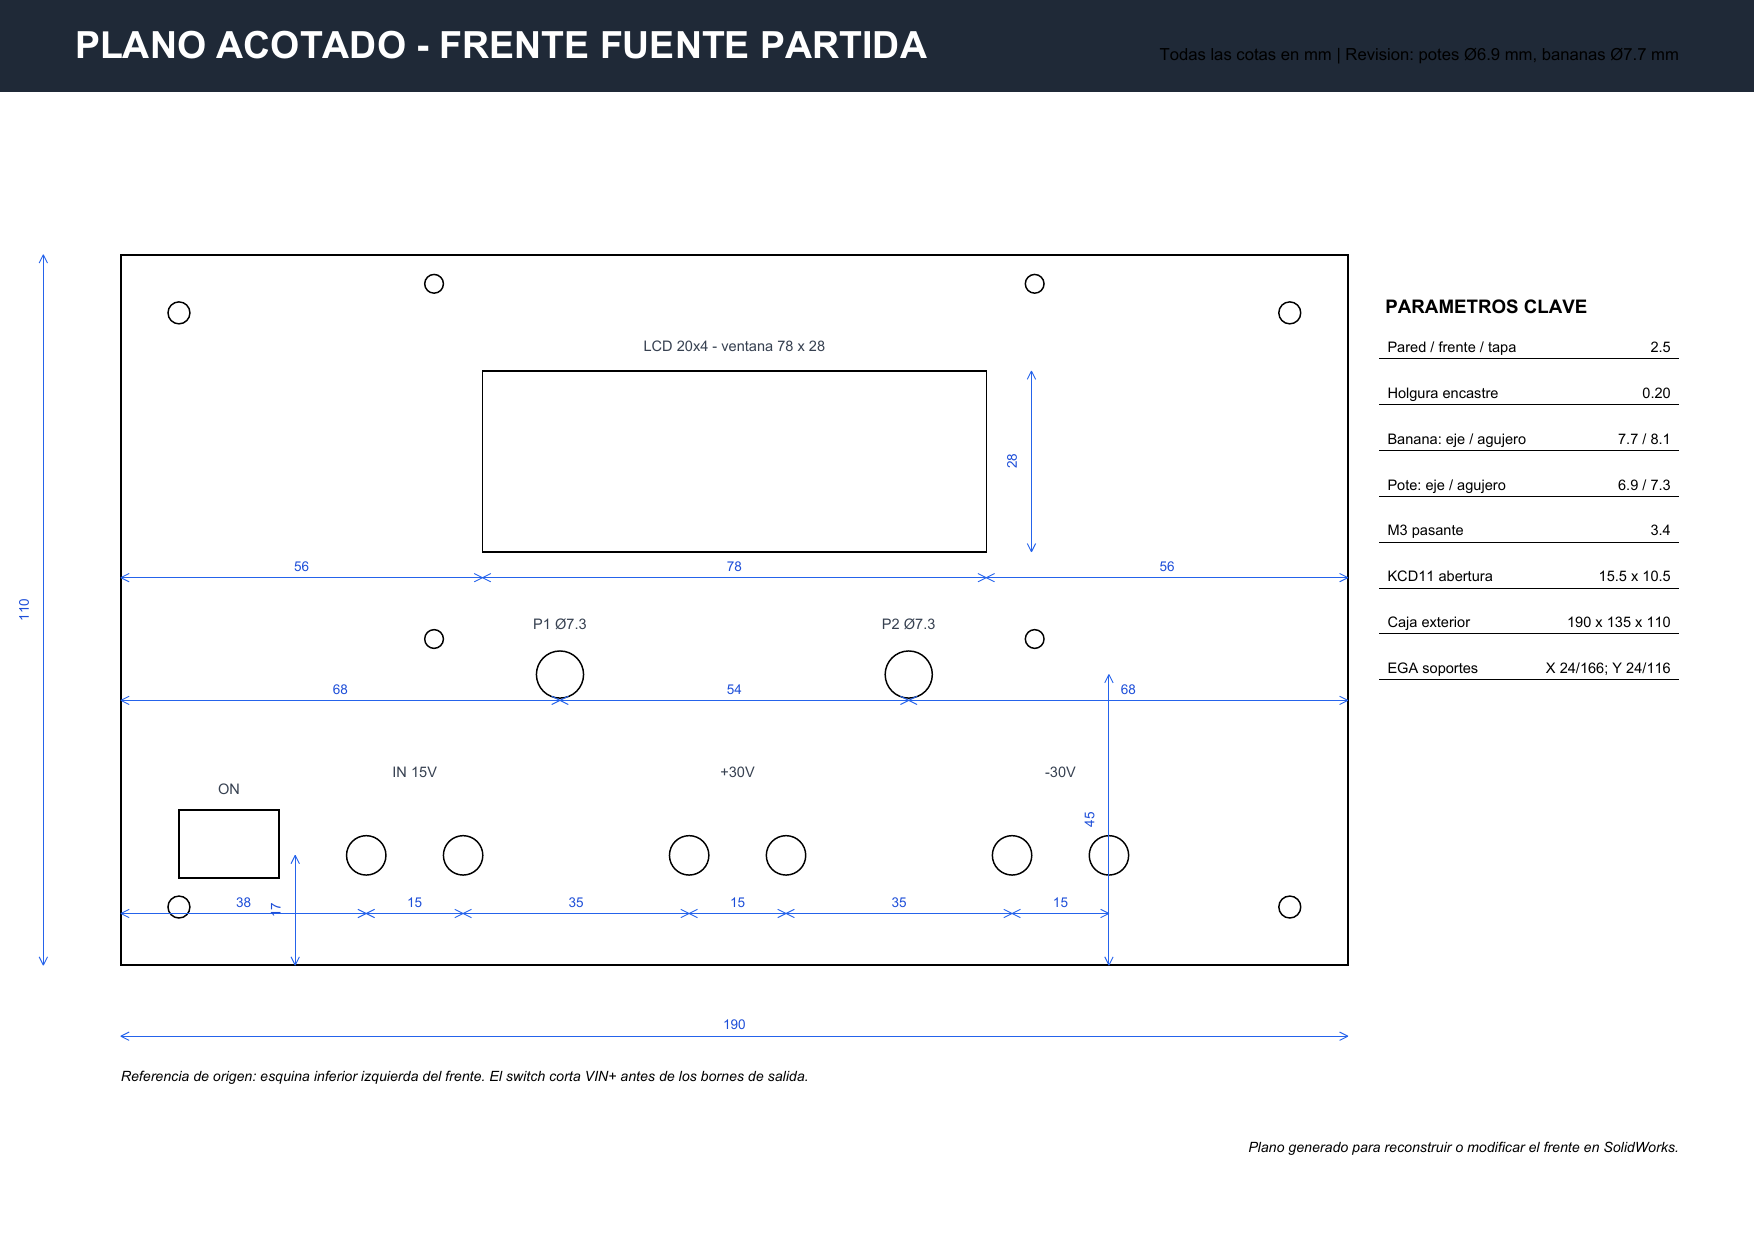
\includegraphics[width=\linewidth,height=0.24\textheight,keepaspectratio]{diseno_frente_3d.png}
\end{minipage}\hfill
\begin{minipage}[c]{0.48\textwidth}
\centering
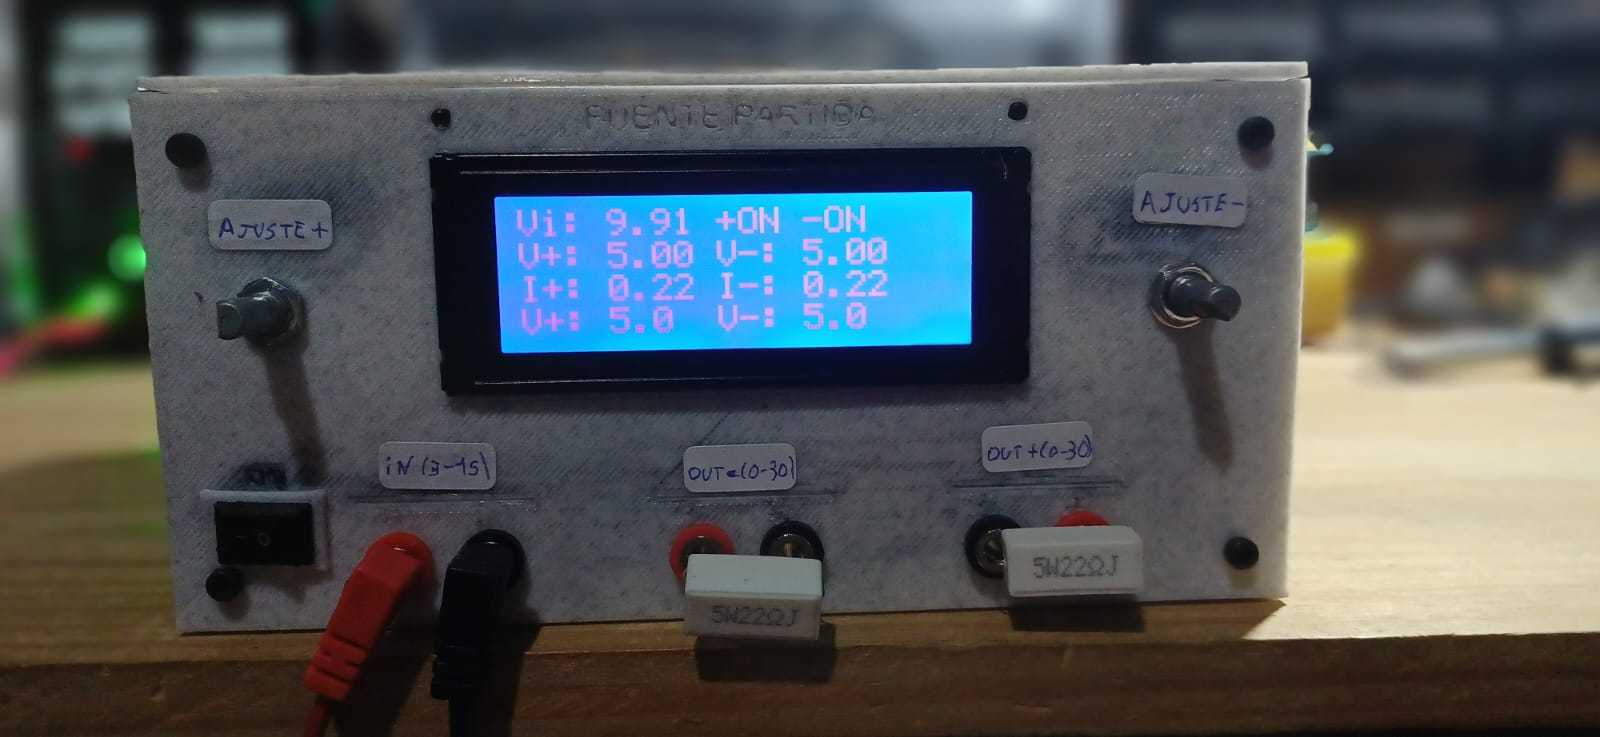
\includegraphics[width=\linewidth,height=0.24\textheight,keepaspectratio]{fuente_carcasa_funcionando.jpeg}
\end{minipage}
\caption{Diseño 3D de la carcasa: plano acotado del frente y prototipo impreso durante el funcionamiento de ambas salidas.}
\label{fig:diseno_3d}
\end{figure*}

%=========================================================
\section{Programación y guía de usuario}

\subsection{Operación mediante encoders}

Al energizar, ambas ramas comienzan apagadas. El encoder izquierdo corresponde a la salida positiva y el derecho a la negativa. El giro cambia el valor activo; una pulsación corta selecciona sucesivamente tensión, corriente límite, sobretensión y PWM; una pulsación larga alterna ON/OFF.

La referencia cambia en pasos de 0,5~V, el límite de corriente en pasos de 0,05~A y la sobretensión en pasos de 0,5~V. El límite de corriente puede ajustarse entre 0,10 y 0,75~A.

\subsection{Lectura del display}

\begin{itemize}
\item Fila 1: Vin y estado ON/OFF de las dos ramas.
\item Fila 2: tensión positiva y magnitud de la tensión negativa.
\item Fila 3: corriente positiva y corriente negativa.
\item Fila 4: parámetro actualmente seleccionado por cada encoder.
\end{itemize}

Si aparece \texttt{OV} o \texttt{OC}, la rama correspondiente queda apagada y la falla permanece enclavada. Después de retirar la causa, una pulsación larga del encoder limpia la indicación sin encender la salida; una segunda pulsación larga vuelve a habilitar la rama.

%=========================================================
\section{Ensayos y resultados}

\subsection{Puesta en marcha por etapas}

La placa se verificó progresivamente. Primero se alimentó únicamente la lógica por USB para comprobar LCD, ADS1115, encoders, UART y PWM sin conectar la etapa de potencia. Después se verificaron las señales de entrada y salida del TC4427. Finalmente se conectaron los transformadores y se habilitó una rama por vez con ciclos pequeños, antes de probar ambas de manera simultánea.

El TC4427 presentó aproximadamente 4,96~V de alimentación y se observaron ambos PWM en sus salidas y en las compuertas de los MOSFET. Esto permitió separar los problemas de lógica de los asociados al transformador, el \textit{snubber} y la carga.

\subsection{Prueba simultánea de las dos ramas y rendimiento}

La prueba final de calibración se realizó con ambas ramas activas al mismo tiempo. Se usaron dos resistencias de 1~k$\Omega$ en paralelo por rama, equivalentes a 500~$\Omega$ por salida. Con 10~V de entrada se alcanzaron aproximadamente +30~V y -30~V. La corriente teórica de carga fue

\begin{equation}
I_o=\frac{30\ \mathrm{V}}{500\ \Omega}\approx60\ \mathrm{mA}
\end{equation}

por rama. La fuente de laboratorio indicó alrededor de 0,468~A de entrada para el funcionamiento conjunto de las dos ramas. La Tabla~\ref{tab:rendimiento} reúne los valores del ensayo.

\begin{table}[!t]
\caption{Ensayo simultáneo de ambas ramas}
\label{tab:rendimiento}
\centering
\footnotesize
\begin{tabular}{@{}ll@{}}
\toprule
\textbf{Magnitud} & \textbf{Valor} \\
\midrule
Tensión de entrada & 10~V \\
Corriente total de entrada & 0,468~A \\
Potencia total de entrada & 4,68~W \\
Salida positiva & +30~V sobre 500~$\Omega$ \\
Salida negativa & -30~V sobre 500~$\Omega$ \\
Corriente por rama & 60~mA \\
Potencia por rama & 1,80~W \\
Potencia total de salida & 3,60~W \\
Rendimiento estimado & 77~\% \\
\bottomrule
\end{tabular}
\end{table}

Con los valores medidos, el rendimiento se estima como

\begin{equation}
\eta\approx\frac{2(30^2/500)}{10(0,468)}\times100\%\approx77\%.
\end{equation}

Cada rama disipó aproximadamente 1,8~W en su carga, es decir, alrededor de 0,9~W por cada resistencia de 1~k$\Omega$. El ensayo se limitó a 30~V debido a la potencia nominal de las cargas utilizadas.

En un ensayo complementario, con 7~V de entrada, 1~k$\Omega$ por rama y ambas salidas funcionando, se alcanzaron aproximadamente 25~V con una corriente de entrada cercana a 0,462~A. Este resultado muestra la dependencia de la tensión máxima respecto de Vin, la carga y la corriente disponible en la entrada.

\subsection{Ensayo de carga de la rama positiva}

La rama positiva se ensayó además con una resistencia cementada de 5~W cuyo valor medido fue 22,2~$\Omega$. Para una salida indicada de 10,0~V, el display mostró 0,45~A. El valor esperado a partir de la carga es

\begin{equation}
I_o=\frac{10,0\ \mathrm{V}}{22,2\ \Omega}=0,450\ \mathrm{A},
\end{equation}

por lo que la indicación coincidió dentro de la resolución de 0,01~A del display. En ese punto la fuente de laboratorio entregó 10~V y 0,634~A, equivalentes a 6,34~W de entrada. La potencia de salida fue aproximadamente 4,50~W y el rendimiento estimado resultó cercano al 71~\%. Los MOSFET se probaron con disipador, mica y tornillo aislado, verificándose previamente la ausencia de continuidad eléctrica entre el transistor y el disipador.

\subsection{Ensayo de carga de la rama negativa}

La rama negativa se ensayó por separado con una resistencia cementada de 5~W cuyo valor medido fue 22,0~$\Omega$. Para una magnitud de salida indicada de 10,0~V, el display mostró 0,45~A, frente a un valor calculado de

\begin{equation}
I_o=\frac{10,0\ \mathrm{V}}{22,0\ \Omega}=0,455\ \mathrm{A}.
\end{equation}

La diferencia fue de 5~mA y quedó dentro de la resolución del display. La fuente de laboratorio indicó 10~V, 0,650~A y aproximadamente 6,497~W. Considerando 4,50~W de salida, el rendimiento estimado de la rama negativa fue cercano al 69~\%.

\subsection{Ensayo EGB con ambas ramas y cargas de 22~$\Omega$}

Como comprobación adicional de la versión EGB se conectaron simultáneamente las resistencias cementadas medidas de 22,2~$\Omega$ y 22,0~$\Omega$. Con la fuente de entrada ajustada a 10,00~V, el instrumento indicó 0,427~A y 4,275~W. Ambas salidas se regularon en 5,00~V y el LCD mostró 0,22~A por rama, valores coherentes con las corrientes calculadas de 0,225~A y 0,227~A.

\begin{table}[!t]
\caption{Ensayo adicional de ambas ramas durante la EGB}
\label{tab:rendimiento_egb}
\centering
\footnotesize
\begin{tabular}{@{}ll@{}}
\toprule
\textbf{Magnitud} & \textbf{Valor} \\
\midrule
Entrada & 10,00~V; 0,427~A; 4,275~W \\
Salida negativa & 5,00~V sobre 22,0~$\Omega$ \\
Salida positiva & 5,00~V sobre 22,2~$\Omega$ \\
Corriente indicada & 0,22~A por rama \\
Potencia total calculada & 2,26~W \\
Rendimiento estimado & 53~\% \\
\bottomrule
\end{tabular}
\end{table}

La potencia de salida se calculó a partir de las resistencias medidas y la tensión indicada:

\begin{equation}
\eta\approx
\frac{5^2/22,0+5^2/22,2}{4,275}\times100\%
\approx53\%.
\end{equation}

Este valor se agrega como un punto de funcionamiento diferente y no reemplaza el rendimiento aproximado de 77~\% obtenido previamente a 30~V con 500~$\Omega$ por rama. La diferencia confirma que el rendimiento depende de la tensión, la corriente, el ciclo de trabajo y las pérdidas de conmutación de cada condición.

\begin{figure*}[!t]
\centering
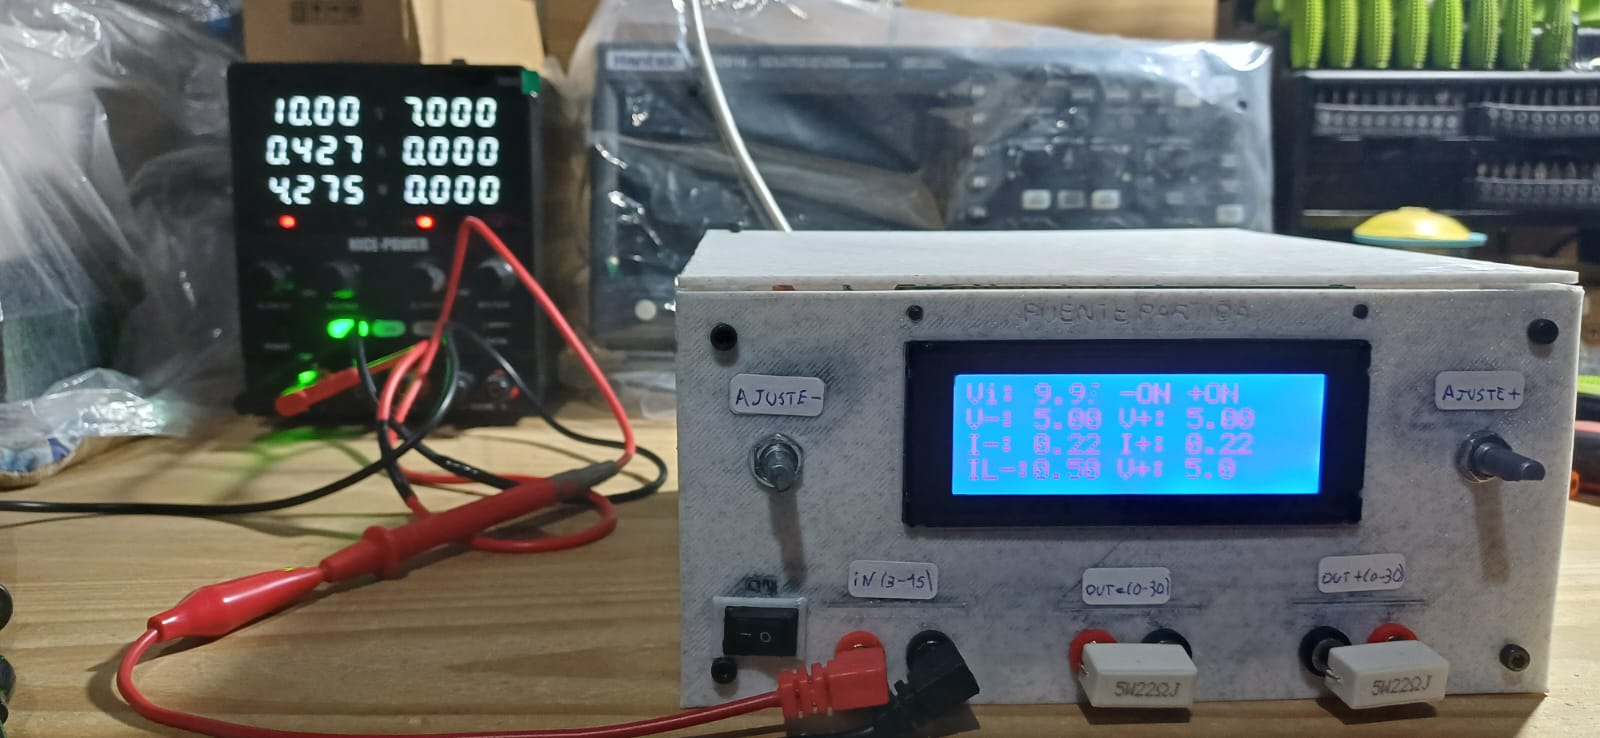
\includegraphics[width=0.92\textwidth,height=0.40\textheight,keepaspectratio]{ensayo_egb_5v_22ohm.jpeg}
\caption{Ensayo EGB con ambas ramas habilitadas, 5,00~V sobre las cargas cementadas de aproximadamente 22~$\Omega$ y medición de 4,275~W en la entrada. El LCD presenta primero la rama negativa y luego la positiva.}
\label{fig:ensayo_egb_5v}
\end{figure*}

\subsection{Resultado de la calibración}

La calibración se implementó mediante tablas independientes para Vin, Vout positiva y la magnitud de Vout negativa. Cada tabla recibe la tensión reconstruida a partir del ADC y entrega el valor corregido que se muestra y utiliza en el control. Al repetir el ensayo se obtuvo coincidencia en la mayoría de los puntos, con un error máximo de tensión de aproximadamente 100~mV alrededor de 12,5~V. En las pruebas resistivas de ambas ramas, la corriente indicada coincidió con el valor calculado dentro de los 10~mA de resolución del display.

\subsection{Margen de error y precisión observada}

La Tabla~\ref{tab:precision} resume por separado la precisión observada en cada rama. Para la tensión se tomó el peor caso registrado en el rango ensayado, mientras que para la corriente se comparó la indicación del display con el valor calculado a partir de la tensión y la resistencia de carga.

\begin{table}[!t]
\caption{Precisión observada en las pruebas}
\label{tab:precision}
\centering
\footnotesize
\begin{tabular}{@{}lcc@{}}
\toprule
\textbf{Rama} & \textbf{Error de tensión} & \textbf{Error de corriente} \\
\midrule
Positiva & $\leq 0,10$~V ($\leq 0,8$~\%) & $<0,01$~A ($<2,2$~\%) \\
Negativa & $\leq 0,10$~V ($\leq 0,8$~\%) & $<0,005$~A ($<1,1$~\%) \\
\bottomrule
\end{tabular}
\end{table}

El display presenta la tensión con una resolución de 0,01~V y la corriente con una resolución de 0,01~A. Por este motivo, en la rama positiva sólo puede afirmarse que el error fue menor que un paso de indicación; en la rama negativa se cuantificó una diferencia de 5~mA. Estos valores representan la precisión observada en las condiciones ensayadas y no una especificación metrológica para todo el rango de operación.

Al medir simultáneamente dos canales con el osciloscopio Hantek DSO2D10 se observó un desplazamiento de aproximadamente 100~mV entre canales aun conectándolos al mismo punto. La autocalibración redujo el error, pero no lo eliminó por completo. Ese valor se tomó como parte de la incertidumbre del instrumento y evita atribuir toda diferencia residual al ADS1115 o al firmware.

\subsection{Verificación de la integración EGB}

La cadena de software se verificó por niveles. En el firmware se comprobó la recepción de órdenes terminadas en nueva línea y la respuesta para consulta, ajuste, habilitación, reinicio de fallas y guardado. En GNU/Linux se verificaron la carga del \textit{overlay}, la asociación del controlador \textit{serdev} y la creación de \texttt{/dev/ega\_uart}. La herramienta de consola y el panel web utilizaron ese mismo dispositivo para consultar y modificar ambas ramas.

También se ejecutaron las pruebas automáticas incluidas con la aplicación web, con resultado satisfactorio en los ocho casos. Estas pruebas cubren la validación de comandos, el análisis de la respuesta \texttt{GET}, el intercambio con el dispositivo y las respuestas de la interfaz HTTP.

%=========================================================
\section{Alternativas evaluadas durante el desarrollo}

Durante el desarrollo se evaluaron configuraciones alternativas a la solución implementada:

\begin{itemize}
\item \textbf{MOSFET sin driver.} Se verificaron la lógica y los PWM con excitación directa desde la Pico. Esta configuración no se adoptó para potencia porque los 3,3~V del GPIO no proporcionan la excitación de compuerta de casi 5~V utilizada con el TC4427.
\item \textbf{Transistores bipolares y Darlingtons.} Se simularon y evaluaron transistores simples, pares complementarios y los Darlingtons 2SD2562/2SB1649. Las necesidades de corriente de base, las pérdidas de saturación y el comportamiento práctico resultaron incompatibles con los objetivos del prototipo. Las simulaciones de LTspice incluidas en los apéndices documentan esta etapa de evaluación.
\item \textbf{Transformador sin núcleo o con una sola E.} Estas configuraciones redujeron fuertemente la inductancia, aumentaron la corriente de entrada y no resolvieron la limitación de tensión. La solución implementada utiliza un núcleo E--E con \textit{gap} total de 1~mm.
\item \textbf{Diferentes capacitores de \textit{snubber}.} El capacitor cerámico 223 se dañó. Se probaron componentes de 10~nF y 33~nF antes de colocar 100~nF/100~V; este último redujo el pico observado.
\end{itemize}

Los resultados obtenidos permitieron identificar las causas de las limitaciones observadas y fundamentaron la selección del driver, los transformadores y la red \textit{snubber} empleados en el prototipo.

%=========================================================
\section{Alcance y limitaciones del prototipo}

Los resultados corresponden a las condiciones ensayadas sobre la placa construida. Los límites relevantes de esta versión son los siguientes:

\begin{itemize}
\item Los MOSFET FQP30N06L poseen una tensión nominal de 60~V y durante los ensayos se observaron picos de VDS cercanos a 40~V con la red \textit{snubber} definitiva.
\item El firmware limita el ciclo de trabajo al 70~\%, valor necesario para alcanzar aproximadamente 30~V en las condiciones ensayadas. El ciclo efectivamente utilizado depende de la tensión de entrada, la referencia y la carga conectada.
\item Los capacitores de salida son de 50~V. La referencia máxima programada es 30~V y el umbral máximo de sobretensión es 40~V.
\item Las protecciones de sobretensión y sobrecorriente son digitales e independientes para cada rama; la PCB implementada no incorpora una protección rápida dedicada por hardware.
\item Se adoptó 0,75~A por rama como límite máximo debido al UF4007. Las mediciones documentadas no incluyen una validación continua a esa corriente ni un ensayo de cortocircuito.
\end{itemize}

%=========================================================
\section{Conclusiones}

La placa integra dos convertidores con transformador, MOSFETs FQP30N06L, driver TC4427, módulo S09, acondicionamiento con MCP6004, ADS1115, Raspberry Pi Pico 2W, dos encoders, LCD, memoria flash y UART. El firmware controla las dos ramas en tareas independientes mediante PI, arranque suave y protecciones digitales por canal.

La calibración por tablas resultó más adecuada que una única ganancia y \textit{offset}, porque corrige la cadena completa de medición después de reconstruir la magnitud eléctrica. Tras la calibración se obtuvo un apartamiento máximo cercano a 0,1~V respecto del osciloscopio en el rango ensayado.

Se demostró el funcionamiento simultáneo hasta aproximadamente $\pm30$~V con una carga de 500~$\Omega$ por rama y 10~V de entrada. En ese punto se estimó un rendimiento aproximado de 77~\%. Como ensayo adicional de la EGB, ambas ramas se probaron simultáneamente a 5,00~V con cargas de 22~$\Omega$; la entrada fue de 10,00~V, 0,427~A y 4,275~W, y el rendimiento total calculado fue cercano al 53~\%. Los dos resultados corresponden a puntos de operación diferentes y no deben interpretarse como un único rendimiento constante. Los ensayos documentados no constituyen una validación continua a 750~mA ni ante cortocircuito.

La EGB completó la integración sin trasladar funciones críticas a Linux. El controlador de carácter encapsula la UART y permite que la consola y el panel web trabajen sobre una interfaz común. La combinación de \texttt{kfifo}, cola de espera, \textit{spinlock} y mutex resuelve la recepción asíncrona y evita la mezcla de transacciones, mientras que el microcontrolador conserva la autoridad final sobre los límites y el estado seguro de las salidas.

%=========================================================
\begin{thebibliography}{00}
\bibitem{b1} Raspberry Pi Ltd., \textit{RP2350 Datasheet}, 2024.
\bibitem{b2} Raspberry Pi Ltd., \textit{Raspberry Pi Pico C/C++ SDK}, 2024.
\bibitem{b3} Texas Instruments, ``ADS1113, ADS1114, ADS1115,'' datasheet.
\bibitem{b4} Microchip Technology, ``TC4426/TC4427/TC4428 MOSFET Drivers,'' datasheet.
\bibitem{b5} onsemi, ``FQP30N06L 60 V Logic N-Channel MOSFET,'' datasheet.
\bibitem{b6} Microchip Technology, ``MCP6001/2/4 Operational Amplifiers,'' datasheet.
\bibitem{b7} R. W. Erickson and D. Maksimovi\'c, \textit{Fundamentals of Power Electronics}, 3rd ed., Springer, 2020.
\bibitem{b8} R. Barry, \textit{Mastering the FreeRTOS Real Time Kernel}, Real Time Engineers Ltd.
\bibitem{b9} The Linux Kernel Documentation, ``Serial device bus,'' documentación de \textit{serdev}.
\bibitem{b10} The Linux Kernel Documentation, ``Generic kernel FIFO implementation,'' documentación de \texttt{kfifo}.
\bibitem{b11} The Linux Kernel Documentation, ``Devicetree usage model,'' documentación del kernel Linux.
\bibitem{web_s09} Sun Cheong Computer Co., ``S09 DC--DC Auto Buck--Boost Converter Module,'' fotografía de producto, disponible en \texttt{scccltd.com}.
\end{thebibliography}

%=========================================================
\onecolumn
\appendices
\clearpage

\begin{landscape}
\section{Diagrama de tareas}

\begin{figure}[!h]
\centering
\resizebox{0.86\linewidth}{!}{%
\begin{tikzpicture}[x=1mm,y=1mm,
  taskbox/.style={draw,rounded corners=1mm,align=left,text width=37mm,minimum width=43mm,minimum height=36mm,inner sep=2mm,font=\small},
  resource/.style={draw,rounded corners=0.8mm,align=center,text width=16mm,minimum width=19mm,minimum height=13mm,inner sep=1mm,fill=gray!16,font=\scriptsize},
  state/.style={resource,fill=yellow!22},
  use/.style={thick,dashed,gray!75},
  flow/.style={-{Latex[length=2.2mm]},thick}]

  \node[taskbox,fill=red!12] (protect) at (-88,58)
    {\textbf{protection\_task} \hfill \textbf{P5}\\[-1mm]
     \rule{37mm}{0.3pt}\\Período: 1 ms.\\
     $\bullet$~Selecciona Vin, I$-$ e I$+$.\\
     $\bullet$~Descarta dos muestras y promedia cuatro.\\
     $\bullet$~Supervisa corriente y caída de Vin.};
  \node[taskbox,fill=red!12] (measure) at (-44,58)
    {\textbf{adc\_task} \hfill \textbf{P3}\\[-1mm]
     \rule{37mm}{0.3pt}\\Período: 5 ms.\\
     $\bullet$~Lee V$+$ y V$-$ con el ADS1115.\\
     $\bullet$~Convierte y calibra magnitudes.\\
     $\bullet$~Publica las mediciones.};
  \node[taskbox,fill=green!18] (display) at (0,58)
    {\textbf{display\_task} \hfill \textbf{P1}\\[-1mm]
     \rule{37mm}{0.3pt}\\Período: 100 ms.\\
     $\bullet$~Copia el estado compartido.\\
     $\bullet$~Actualiza las cuatro filas del LCD.\\
     $\bullet$~Muestra fallas enclavadas.};
  \node[taskbox,fill=blue!14] (encoder) at (44,58)
    {\textbf{encoder\_task} \hfill \textbf{P3}\\[-1mm]
     \rule{37mm}{0.3pt}\\Período: 1 ms.\\
     $\bullet$~Lee los dos encoders KY-040.\\
     $\bullet$~Modifica el ajuste seleccionado.\\
     $\bullet$~Habilita o apaga cada rama.};
  \node[taskbox,fill=green!18] (uart) at (88,58)
    {\textbf{uart\_task} \hfill \textbf{P2}\\[-1mm]
     \rule{37mm}{0.3pt}\\Período: 2 ms.\\
     $\bullet$~Recibe comandos por UART0.\\
     $\bullet$~Consulta o cambia cada rama.\\
     $\bullet$~Ordena el guardado en flash.};

  % Recursos de acceso directo, alineados en una fila.
  \node[resource] (adc) at (-99,22) {ADC FIFO\\e IRQ};
  \node[resource] (i2c) at (-22,22) {I$^2$C0\\mutex};
  \node[resource] (flash) at (52,22) {Flash\\interna};
  \node[resource] (uartres) at (99,22) {UART0\\GPIO0/1};
  \node[state,text width=21mm,minimum width=24mm] (shared) at (0,0) {Estado\\compartido};

  \draw[use] ([xshift=-10mm]protect.south) -- (adc.north);
  \draw[use] ([xshift=10mm]measure.south) -- (-34,31) -- (-22,31) -- (i2c.north);
  \draw[use] ([xshift=-10mm]display.south) -- (-10,31) -- (-22,31);
  \fill[gray!75] (-22,31) circle (1mm);
  \draw[use] ([xshift=-10mm]uart.south) -- (72,31) -- (52,31) -- (flash.north);
  \fill[gray!75] (52,31) circle (1mm);
  \draw[use] ([xshift=12mm]uart.south) -- (uartres.north);

  % Troncal superior del estado compartido.
  \draw[use] (shared.north) -- (0,10);
  \draw[use] (-88,10) -- (88,10);
  \draw[use] (protect.south) -- (-88,10);
  \draw[use] (measure.south) -- (-44,10);
  \draw[use] (display.south) -- (0,10);
  \draw[use] (encoder.south) -- (44,10);
  \draw[use] (uart.south) -- (88,10);
  \foreach \x in {-88,-44,0,44,88} {\fill[gray!75] (\x,10) circle (1mm);}

  \node[taskbox,fill=orange!24] (controlp) at (-30,-43)
    {\textbf{control\_task (+)} \hfill \textbf{P4}\\[-1mm]
     \rule{37mm}{0.3pt}\\Período: 5 ms.\\
     $\bullet$~Aplica el arranque suave positivo.\\
     $\bullet$~Calcula el PI con V$+$.\\
     $\bullet$~Actualiza PWM\_POS.};
  \node[taskbox,fill=orange!24] (controln) at (30,-43)
    {\textbf{control\_task (-)} \hfill \textbf{P4}\\[-1mm]
     \rule{37mm}{0.3pt}\\Período: 5 ms.\\
     $\bullet$~Aplica el arranque suave negativo.\\
     $\bullet$~Calcula el PI con V$-$.\\
     $\bullet$~Actualiza PWM\_NEG.};
  \node[resource] (pwmp) at (-30,-73) {PWM\_POS\\GPIO16};
  \node[resource] (pwmn) at (30,-73) {PWM\_NEG\\GPIO17};

  \draw[use] (shared.south) -- (0,-17);
  \draw[use] (-30,-17) -- (30,-17);
  \draw[use] (controlp.north) -- (-30,-17);
  \draw[use] (controln.north) -- (30,-17);
  \foreach \x in {-30,0,30} {\fill[gray!75] (\x,-17) circle (1mm);}
  \draw[flow] (controlp.south) -- (pwmp.north);
  \draw[flow] (controln.south) -- (pwmn.north);
\end{tikzpicture}}
\caption{Siete tareas de FreeRTOS y recursos compartidos. \texttt{protection\_task} estabiliza la selección de canales y supervisa Vin; el corte de sobrecorriente se ejecuta directamente en la IRQ del ADC. Las líneas discontinuas indican acceso a un recurso y las flechas continuas corresponden a las salidas PWM.}
\label{fig:tareas}
\end{figure}
\end{landscape}

\clearpage
\begin{landscape}
\section{Diagrama en bloques}

\begin{figure}[!h]
\centering
\resizebox{0.88\linewidth}{!}{%
\begin{tikzpicture}[x=1mm,y=1mm,
  block/.style={draw,align=center,text width=29mm,minimum height=17mm,inner sep=2mm,font=\small},
  pico/.style={block,text width=44mm,minimum height=31mm,fill=red!15},
  bus/.style={block,text width=31mm,minimum height=19mm,fill=green!12},
  arrow/.style={-{Latex[length=2.4mm]},thick},
  both/.style={{Latex[length=2.2mm]}-{Latex[length=2.2mm]},thick},
  signal/.style={-{Latex[length=2.2mm]},thick,dashed},
  pin/.style={font=\scriptsize,align=center,fill=white,inner sep=1mm}]

  \node[block,fill=orange!20] (j1) at (-112,68) {Entrada J1\\VCC 3,7--15 V};
  \node[block,fill=orange!20] (s09) at (-68,68) {U4 S09 / B6285\\salida auxiliar +5 V};
  \node[pico] (pico) at (-14,22) {\textbf{Raspberry Pi Pico 2W}\\FreeRTOS -- 7 tareas\\ADC -- PWM -- I$^2$C0 -- UART0};
  \node[block,fill=orange!22,text width=29mm,minimum height=25mm] (driver) at (38,22) {\textbf{TC4427}\\driver dual\\VDD: pin 6};
  \node[block,fill=blue!16] (pos) at (88,48) {Rama positiva\\Q1 -- TR1 -- D1};
  \node[block,fill=cyan!16,text width=24mm] (outp) at (132,48) {Salida J2\\VOUT\_POS};
  \node[block,fill=blue!16] (neg) at (88,-4) {Rama negativa\\Q2 -- TR2 -- D4};
  \node[block,fill=cyan!16,text width=24mm] (outn) at (132,-4) {Salida J6\\VOUT\_NEG};

  \node[block,fill=gray!18] (usb) at (-112,36) {Conector USB\\programación};
  \node[block,fill=green!16] (uart) at (-112,12) {Conector J13\\UART hacia otra placa};
  \node[block,fill=green!16] (enc) at (-112,-12) {Dos encoders KY-040\\positivo y negativo};
  \node[block,fill=green!16] (lcd) at (-112,-46) {LCD 20$\times$4\\módulo PCF8574};
  \node[bus] (i2cbus) at (-66,-46) {\textbf{Bus I$^2$C0}\\SDA: GPIO12\\SCL: GPIO13};
  \node[block,fill=yellow!20] (ads) at (-16,-68) {ADS1115\\VDD: 3V3 (pin 36)};
  \node[block,fill=yellow!20,text width=37mm] (mcp) at (44,-68) {MCP6004\\VDD: 3V3 (pin 36)};

  % Alimentación y lectura de entrada.
  \draw[arrow] (j1.east) -- node[pin,above]{VCC / GND} (s09.west);
  \draw[arrow] (s09.south) -- (-68,47) -- node[pin,above]{+5 V / VSYS (39)} (-14,47) -- (pico.north);
  \draw[arrow] (s09.north) -- (-68,82) -- node[pin,above]{+5 V / VDD (6)} (38,82) -- (driver.north);
  \draw[signal] (j1.south) -- (-112,54) -- node[pin,above]{VIN\_SENSE / GPIO26 ADC0} (-42,54) -- (-42,30) -- ([yshift=8mm]pico.west);

  % Interfaces de usuario y comunicación.
  \draw[arrow] (usb.east) -- node[pin,above]{VBUS / pin 40} (-44,36) -- (-44,28) -- ([yshift=6mm]pico.west);
  \draw[both] (uart.east) -- node[pin,above]{GPIO0 TX / GPIO1 RX} (-44,12) -- (-44,18) -- ([yshift=-4mm]pico.west);
  \draw[arrow] (enc.east) -- node[pin,below]{POS: GPIO2/3/4 \quad NEG: GPIO6/7/8} (-42,-12) -- (-42,8) -- ([yshift=-14mm]pico.west);
  \draw[both] (lcd.east) -- node[pin,above]{SDA / SCL} (i2cbus.west);
  \draw[both] (i2cbus.north) -- (-66,-28) -- node[pin,above]{SDA GPIO12 / SCL GPIO13} (-14,-28) -- (pico.south);
  \draw[both] (i2cbus.south) -- (-66,-68) -- node[pin,above]{SDA / SCL} (ads.west);

  % PWM y etapas de potencia.
  \draw[arrow] ([yshift=6mm]pico.east) -- node[pin,above]{GPIO16 / INA (2)} ([yshift=6mm]driver.west);
  \draw[arrow] ([yshift=-6mm]pico.east) -- node[pin,below]{GPIO17 / INB (4)} ([yshift=-6mm]driver.west);
  \draw[arrow] ([yshift=6mm]driver.east) -- (68,28) -- (68,48) -- node[pin,above]{OUTA (7) / Gate Q1} (pos.west);
  \draw[arrow] ([yshift=-6mm]driver.east) -- (68,16) -- (68,-4) -- node[pin,below]{OUTB (5) / Gate Q2} (neg.west);
  \draw[arrow] (pos.east) -- (outp.west);
  \draw[arrow] (neg.east) -- (outn.west);

  % Realimentación analógica por recorridos ortogonales independientes.
  \draw[signal] (outp.east) -- (158,48) -- (158,-42) -- node[pin,above]{VOUT\_POS / RSHUNT1} (44,-42) -- (mcp.north);
  \draw[signal] (outn.east) -- (151,-4) -- (151,-53) -- node[pin,above]{VOUT\_NEG / RSHUNT2} (66,-53) -- (66,-68) -- (mcp.east);
  \draw[signal] (mcp.west) -- (ads.east)
    node[pin,above,pos=0.50]{Vout$+$ / AIN0}
    node[pin,below,pos=0.50]{Vout$-$ / AIN1};
  \draw[signal] (mcp.north) -- (44,-31) -- node[pin,above]{I$+$ GPIO28 ADC2 / I$-$ GPIO27 ADC1} (12,-31) -- (12,7) -- (pico.south east);
\end{tikzpicture}}
\caption{Conexión de los módulos y pines utilizados. Las líneas continuas representan alimentación o señales digitales; las discontinuas corresponden a mediciones analógicas.}
\label{fig:bloques_detallado}
\end{figure}
\end{landscape}

\clearpage
\begin{landscape}
\section{Ensayo de banco durante la calibración}
\begin{figure}[!h]
\centering
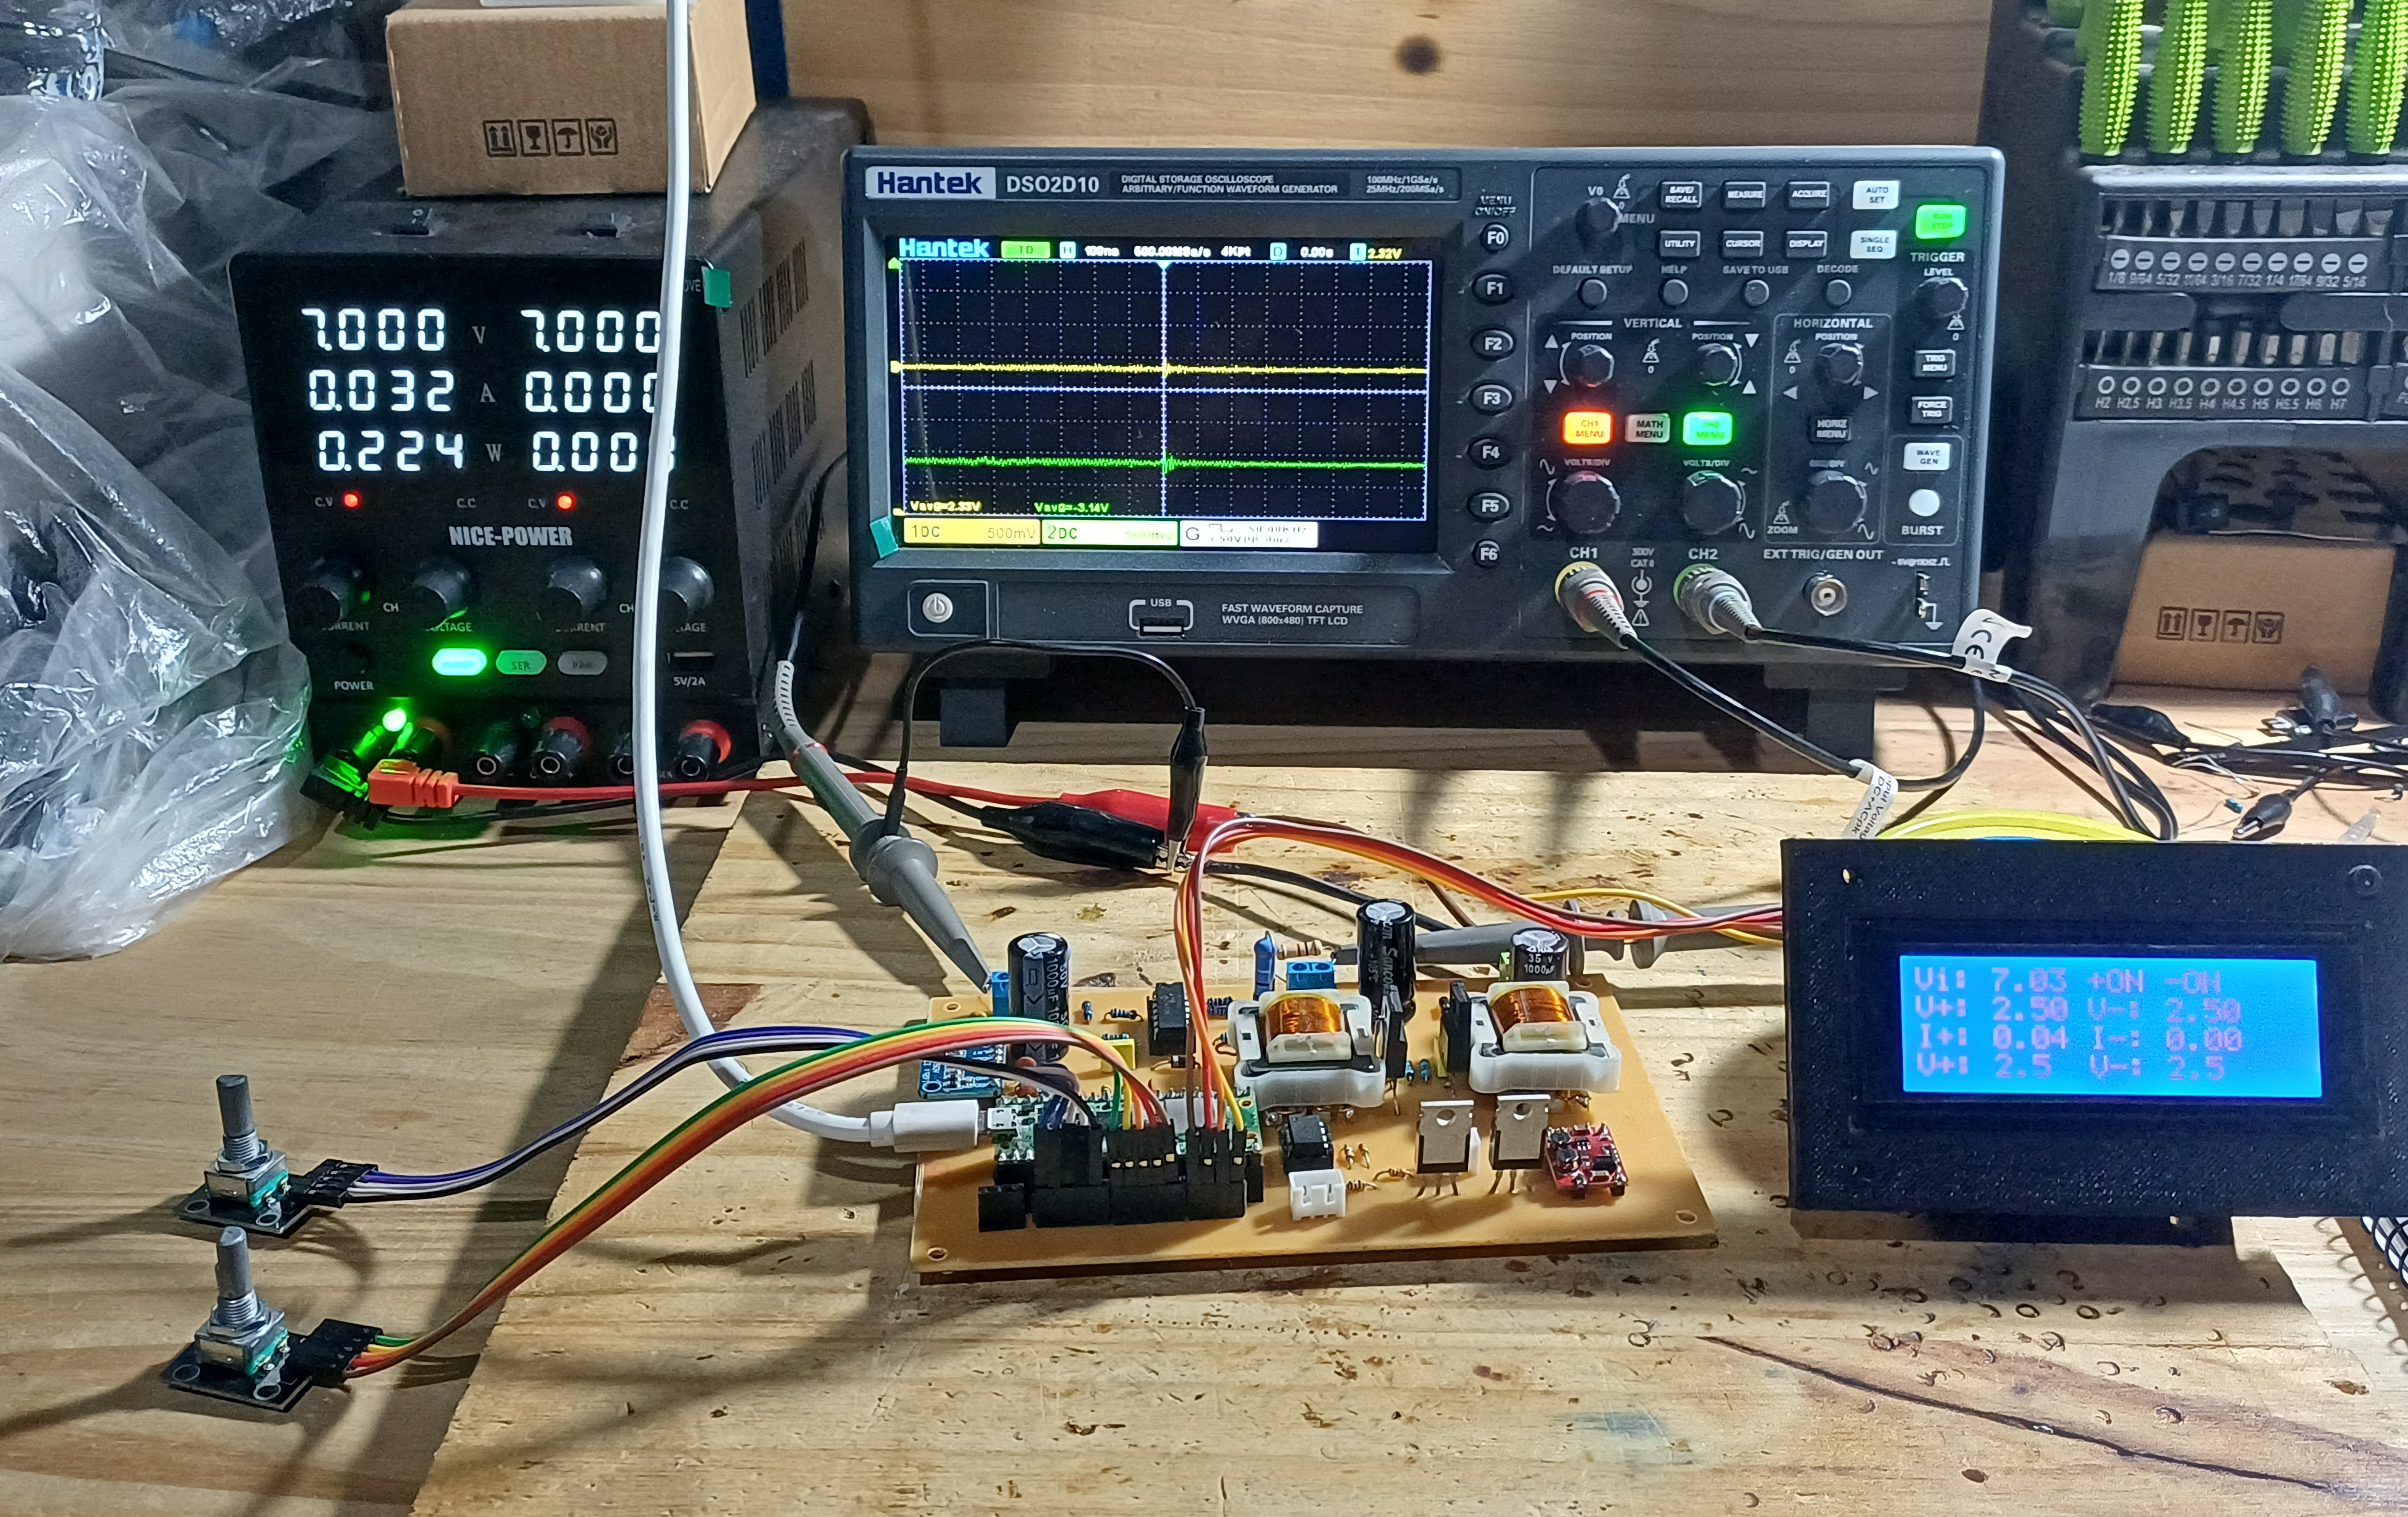
\includegraphics[width=0.98\linewidth,height=0.82\textheight,keepaspectratio]{20260914_121951.jpg}
\caption{Prototipo completo durante el proceso de calibración. Se observan las dos cargas, los encoders, el LCD, la fuente de laboratorio y los dos canales del osciloscopio Hantek DSO2D10. Las diferencias medidas entre el instrumental y el display se utilizaron para obtener las tablas independientes de Vin, Vout positiva y Vout negativa.}
\label{fig:antes_calibracion}
\end{figure}
\end{landscape}

\clearpage
\begin{landscape}
\section{Esquemático implementado}
\begin{figure}[!h]
\centering
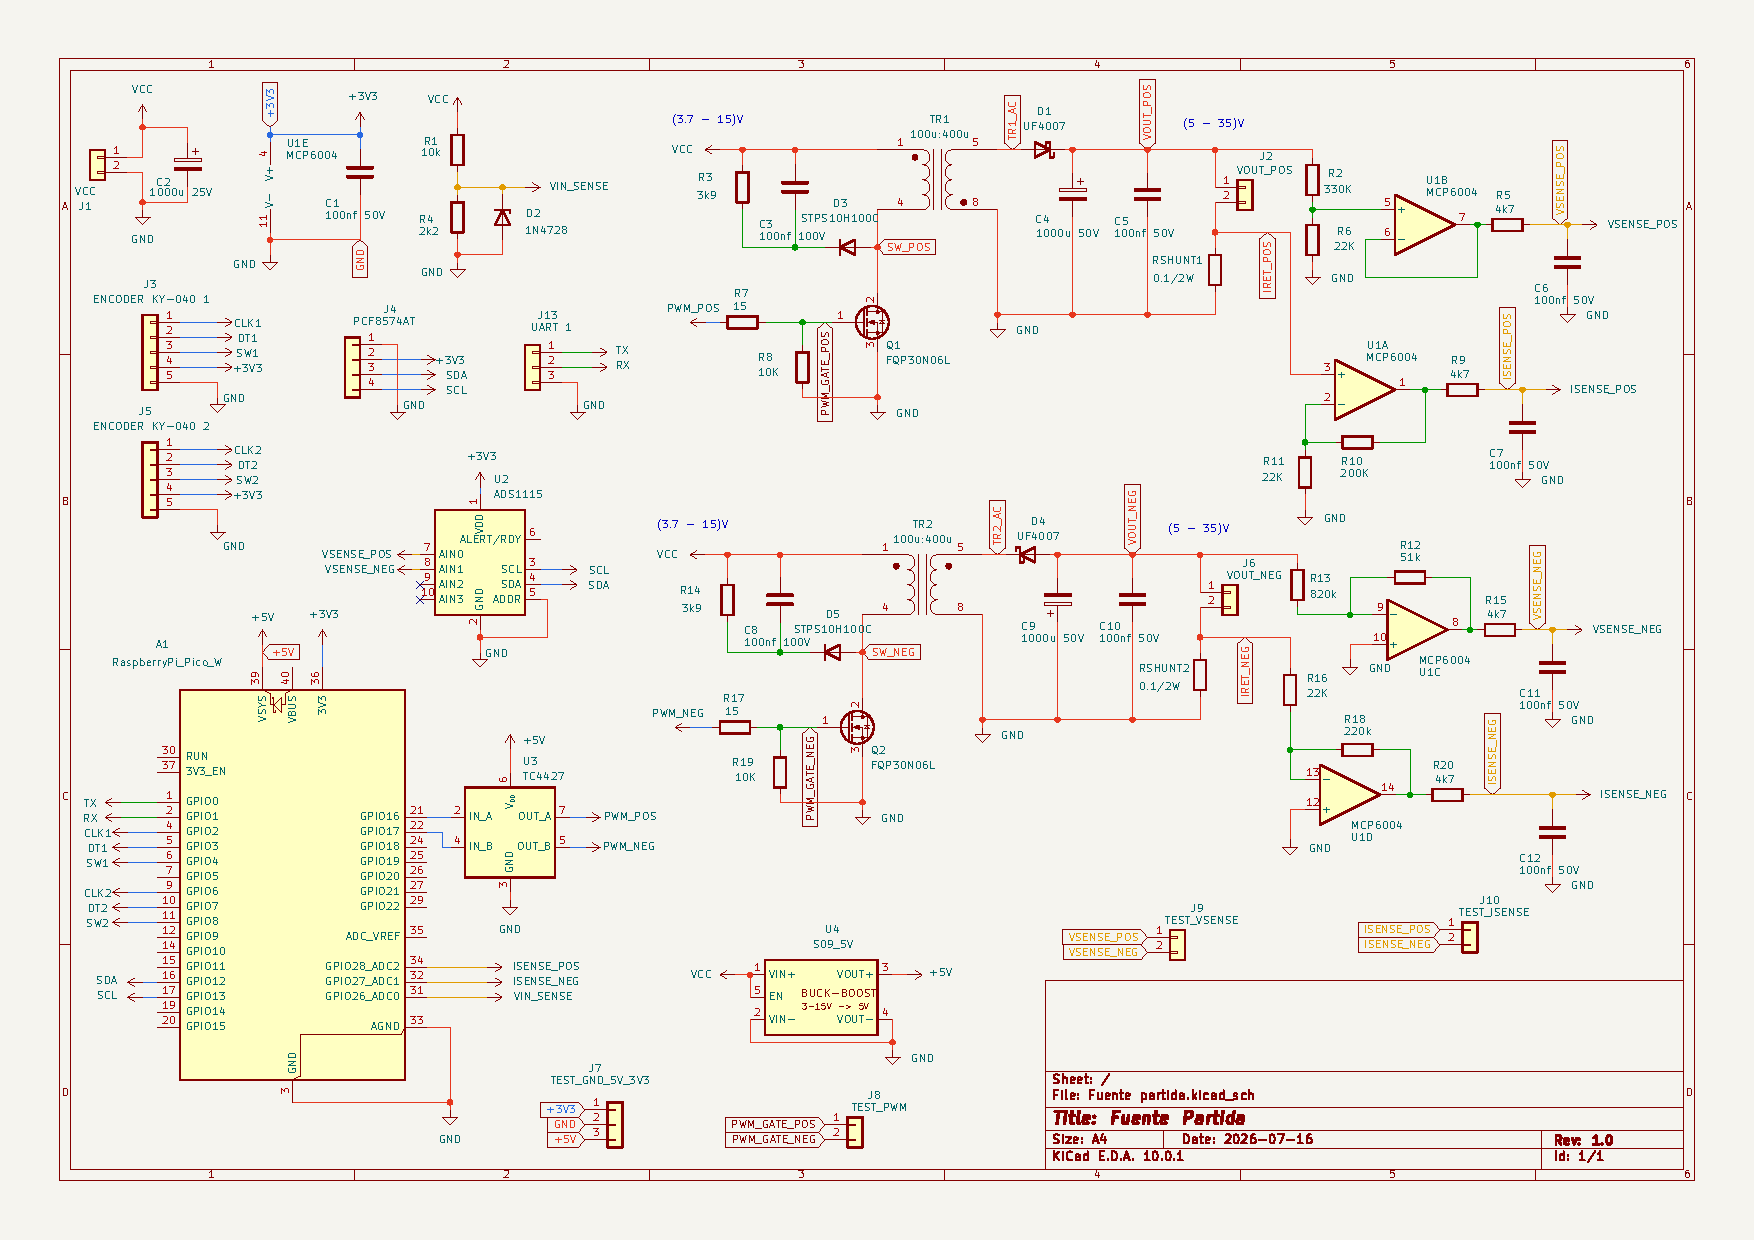
\includegraphics[width=0.98\linewidth,height=0.82\textheight,keepaspectratio]{esquematico_color.pdf}
\caption{Esquemático completo a color exportado desde el proyecto KiCad de la placa implementada.}
\label{fig:esquematico}
\end{figure}
\end{landscape}

\clearpage
\begin{landscape}
\section{PCB -- vista superior}
\begin{figure}[!h]
\centering
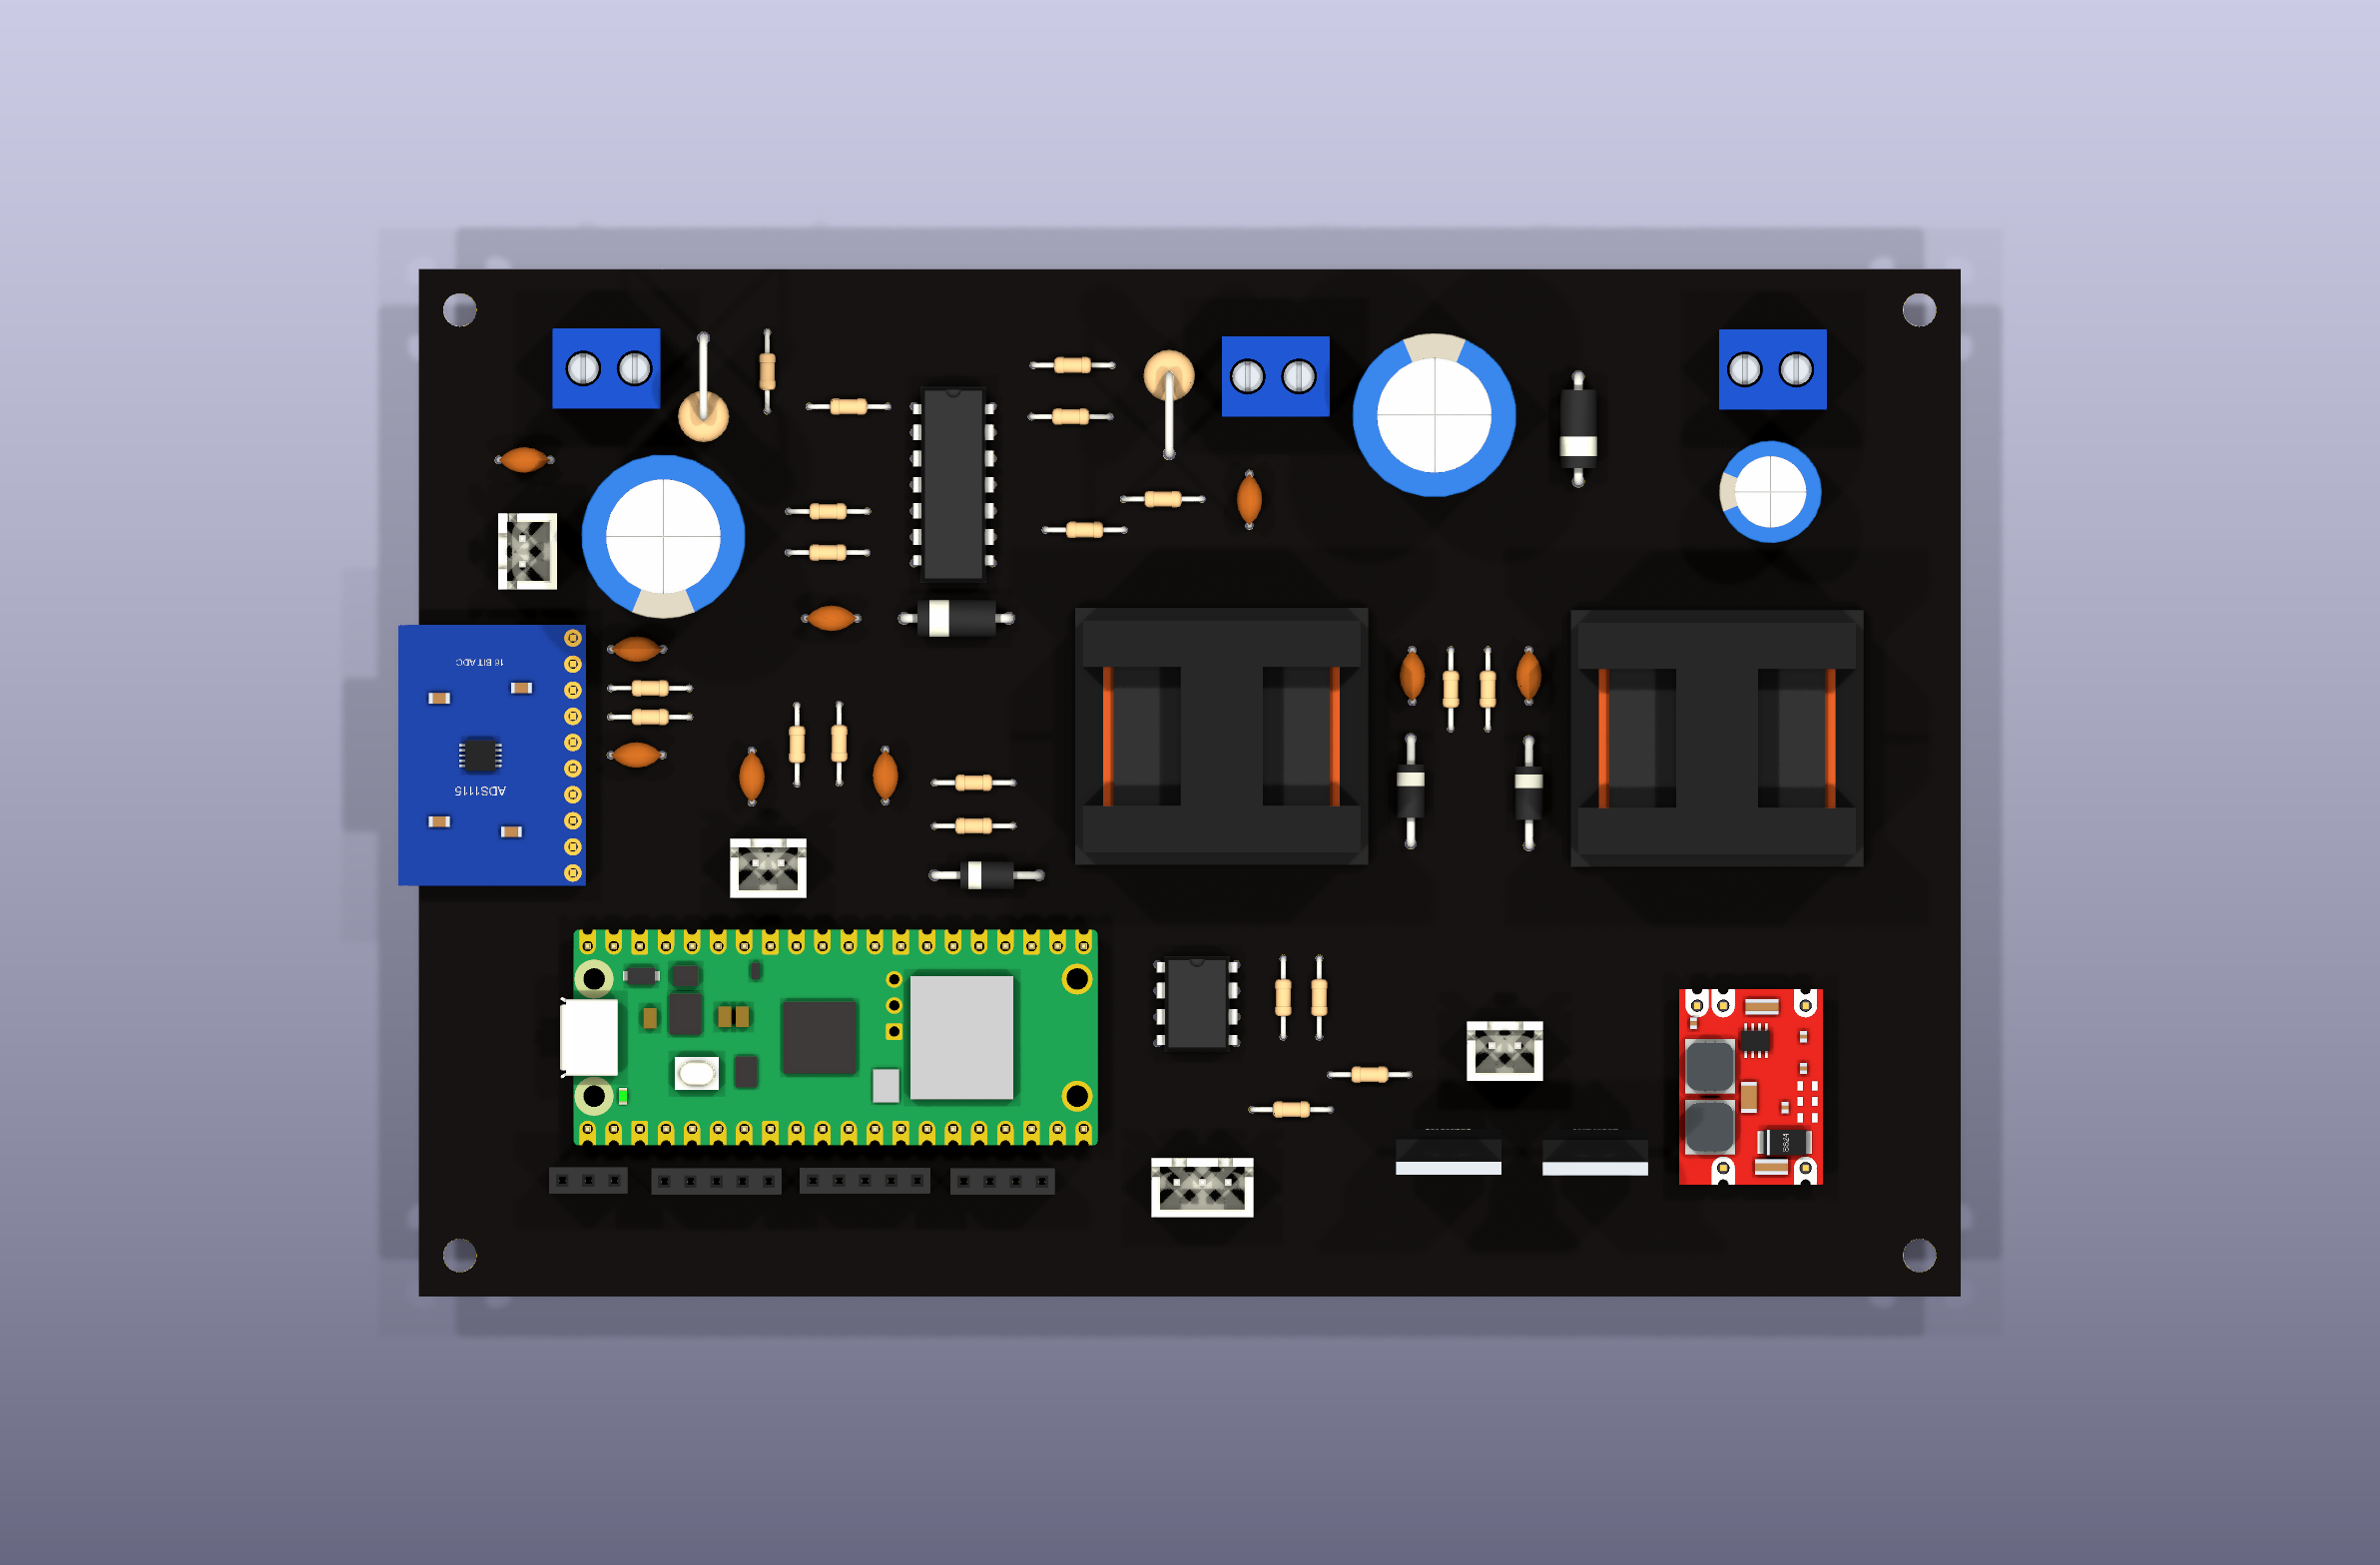
\includegraphics[width=0.98\linewidth,height=0.82\textheight,keepaspectratio]{pcb_top.png}
\caption{Vista superior completa de la PCB implementada de 150~mm por 100~mm.}
\label{fig:pcbtop}
\end{figure}
\end{landscape}

\clearpage
\begin{landscape}
\section{PCB -- vista inferior}
\begin{figure}[!h]
\centering
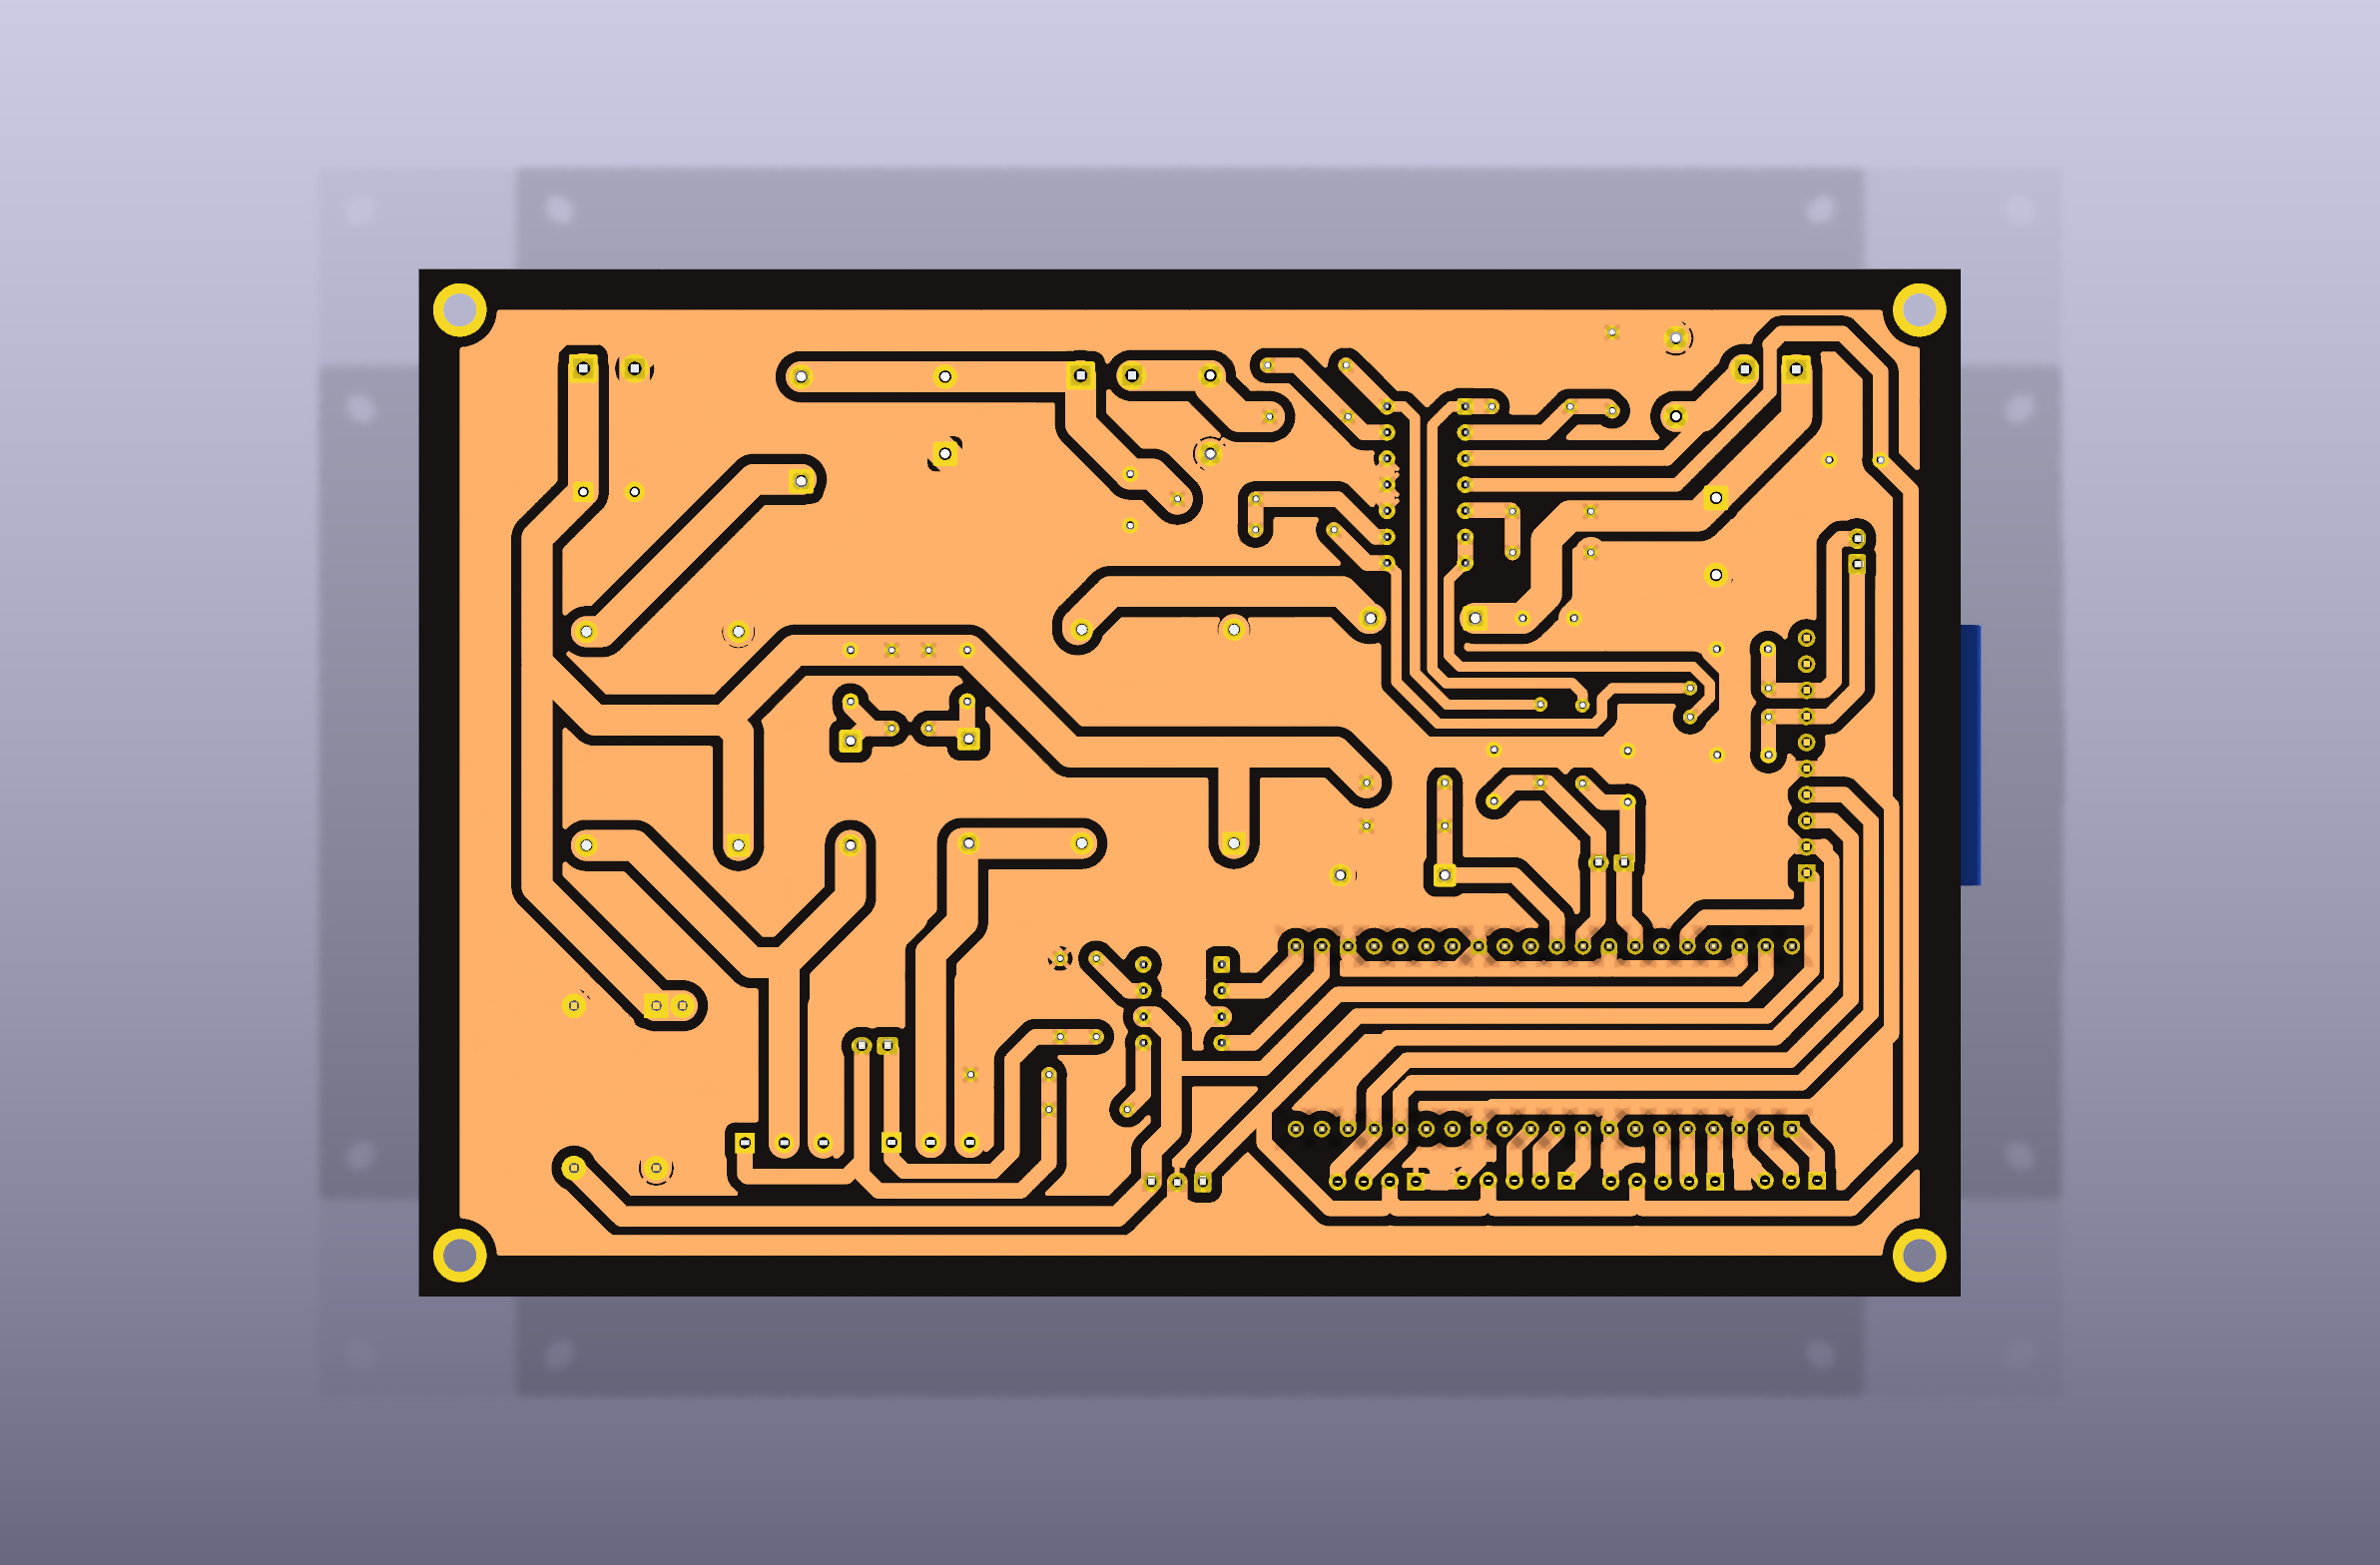
\includegraphics[width=0.98\linewidth,height=0.82\textheight,keepaspectratio]{pcb_bottom.png}
\caption{Capa B.Cu exportada desde KiCad, con el ruteo de cobre y los taladros de la PCB implementada.}
\label{fig:pcbbottom}
\end{figure}
\end{landscape}

\clearpage
\begin{landscape}
\section{Simulación de una alternativa a 15 V}
\begin{figure}[!h]
\centering
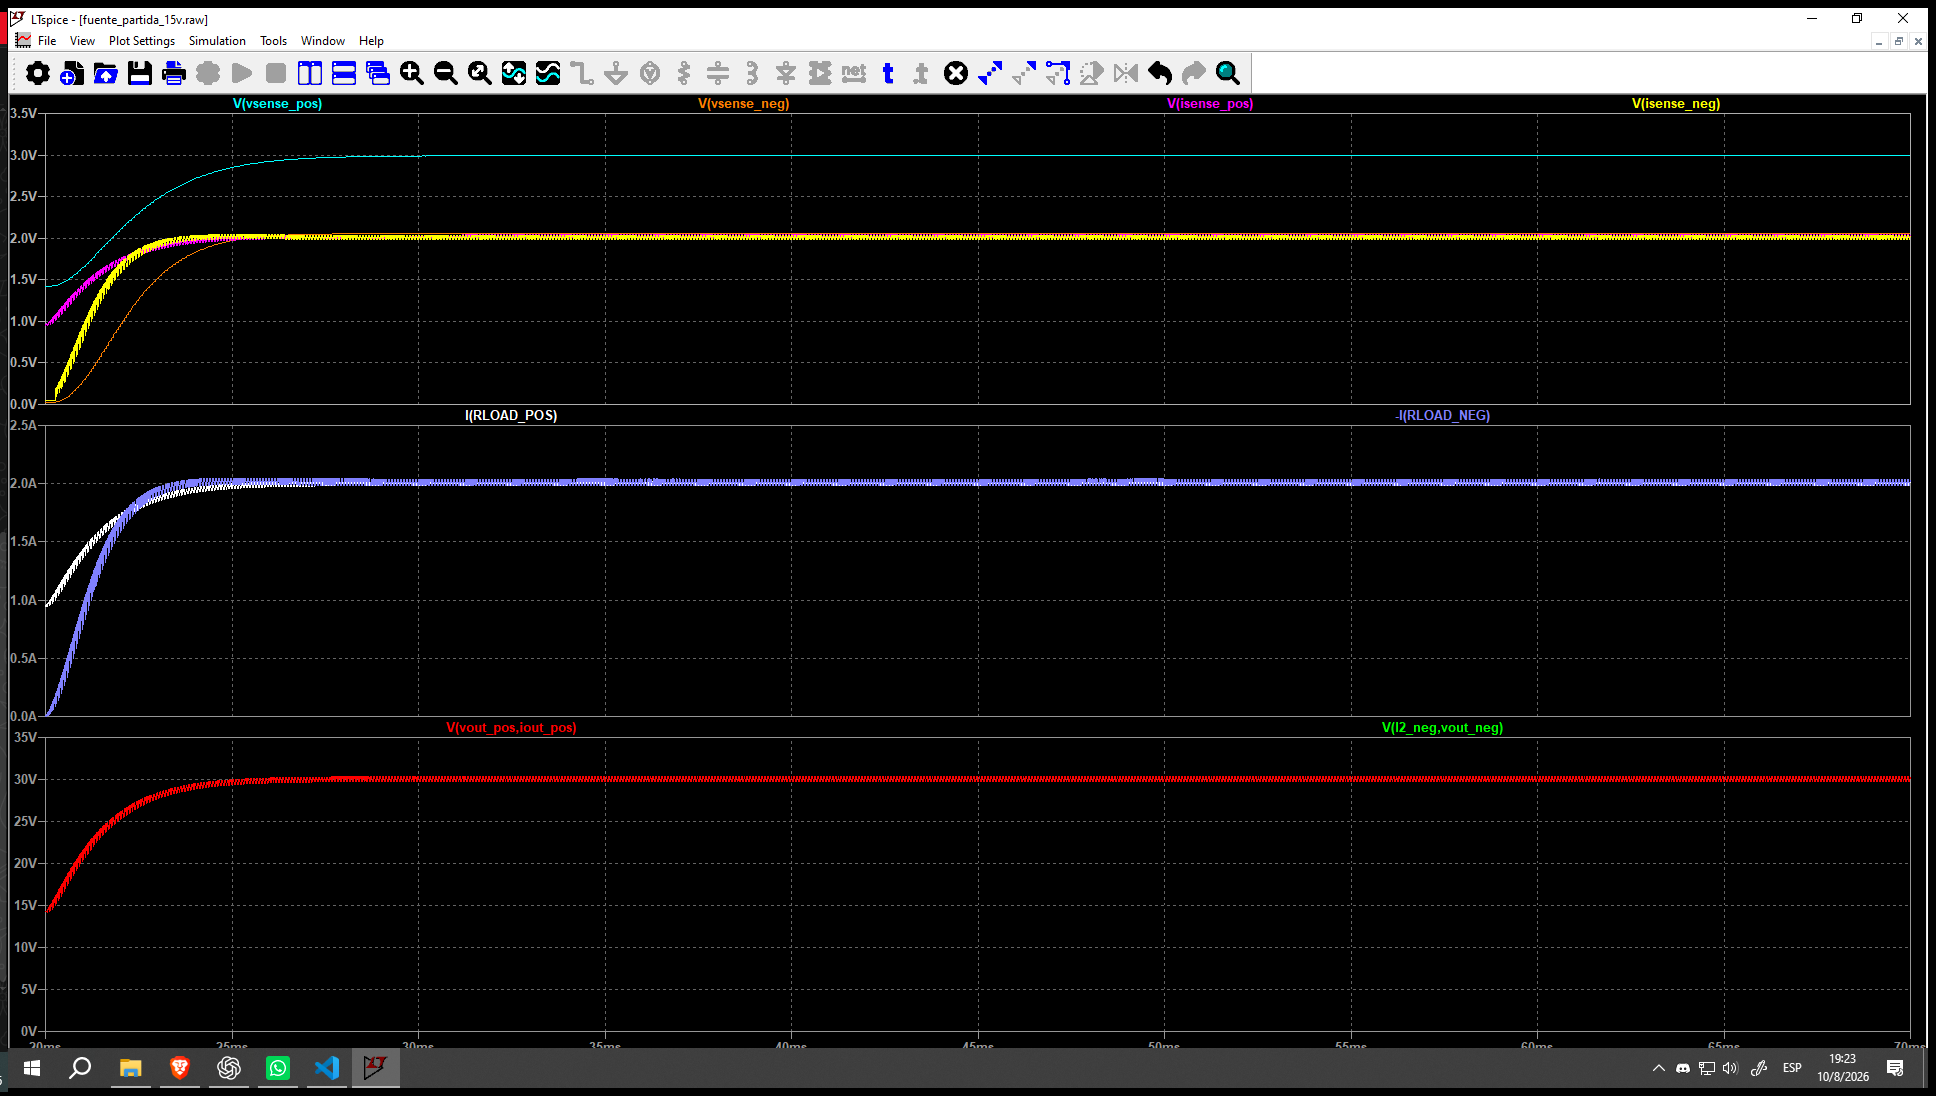
\includegraphics[width=0.98\linewidth,height=0.82\textheight,keepaspectratio]{captura_ltspice_15v.png}
\caption{Simulación correspondiente a una alternativa evaluada antes de seleccionar la etapa de potencia con FQP30N06L y TC4427.}
\label{fig:ltspice15}
\end{figure}
\end{landscape}

\clearpage
\begin{landscape}
\addcontentsline{toc}{section}{Apéndice H: Simulación de una alternativa a 3,7 V}
\begin{center}
{\normalsize\scshape Apéndice H\\[2pt]Simulación de una alternativa a 3,7 V}
\end{center}
\begin{figure}[!h]
\centering
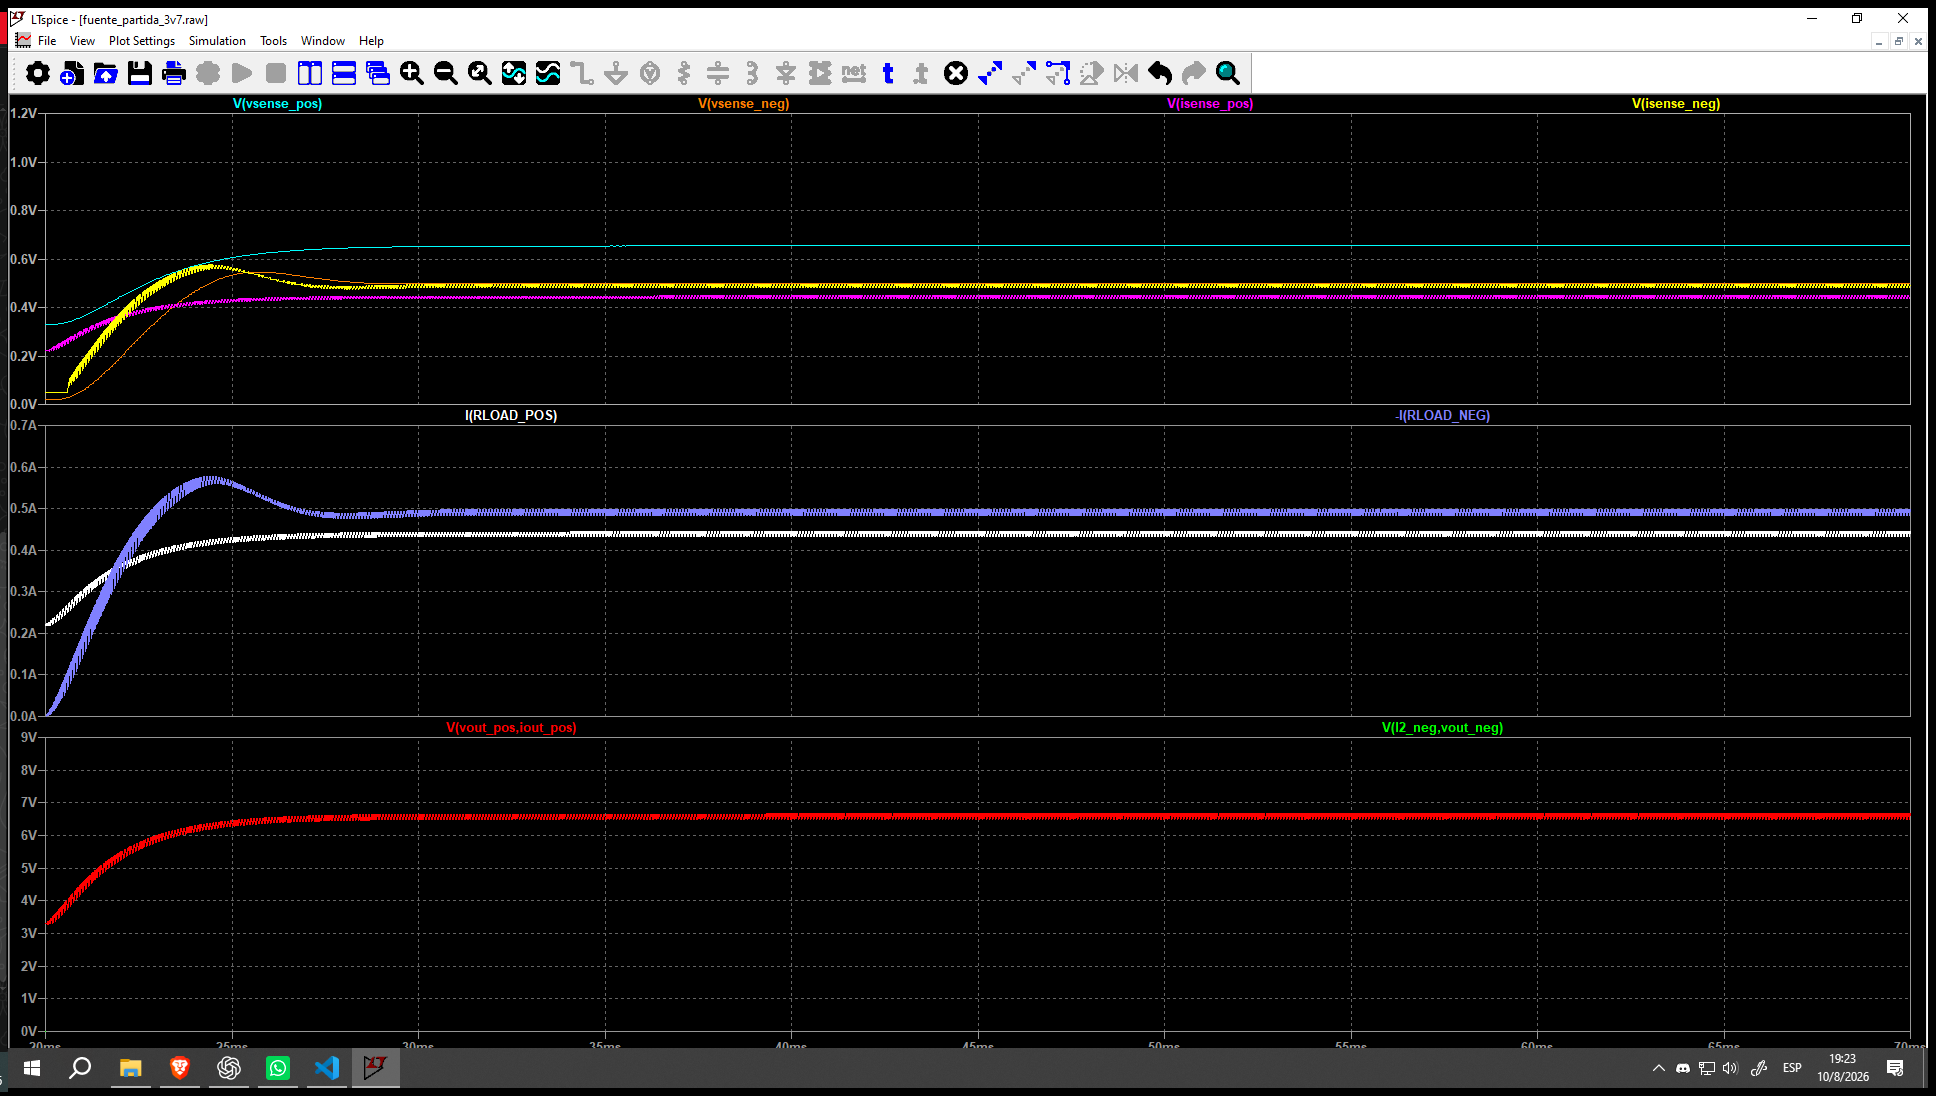
\includegraphics[width=0.98\linewidth,height=0.82\textheight,keepaspectratio]{captura_ltspice_3v7.png}
\caption{Simulación correspondiente a una de las configuraciones evaluadas durante el desarrollo.}
\label{fig:ltspice37}
\end{figure}
\end{landscape}

\end{document}
